%----------------------------------------
\documentclass[aps, prl]{revtex4-2}  % for review and submission
\usepackage{comment}
\usepackage{graphicx}  % needed for figures
\usepackage{ragged2e}
\usepackage{dcolumn}   % needed for some tables
\usepackage{bm}        % for math
\usepackage{amssymb}   % for math
\usepackage{amsmath}   % for math
\usepackage[top=0.85in,left=0.9in, right=0.9in, bottom=0.9in]{geometry}
\usepackage[hidelinks]{hyperref}
\usepackage{fancyhdr}
\usepackage{xcolor}
\usepackage{float}
\usepackage{lipsum}
\usepackage[compact]{titlesec}

\hypersetup{
    colorlinks,
    linkcolor={blue!80!black},
    citecolor={blue!80!black},
    urlcolor={blue!80!black}
}
% avoids incorrect hyphenation, added Nov/08 by SSR
\hyphenation{ALPGEN}
\hyphenation{EVTGEN}
\hyphenation{PYTHIA}
%

\begin{document}
\title{Supplementary Materials: Probing the Deuteron at Very Large Internal Momenta}
\maketitle
\section{\large Event Selection Cuts}
\indent Figures \ref{fig:Em_Q2_cuts}-\ref{fig:simc_coll_cuts} show the event selection cuts for data (blue hatched) and SIMC (red data points) for the deuteron 80 MeV/c kinematic setting at $\theta_{nq}=35\pm5^{\circ}$.
The black dashed or red solid lines (for collimators) represent the cuts or geometrical (collimators) boundaries used to select true $^{2}$H$(e,e'p)n$ coincidence events.
The exact same cuts were also applied to the 580 and 750 MeV/c settings. Each histogram has all the other event selection cuts described except a self cut.
The integrated counts (within the cut boundary) for data and simulation as well as the data-to-simulation yield ratio is shown (top left) for each selection cut.
The data yield has been normalized by the total charge and corrected for the inefficiencies described in the Letter. The FSI model from J.M. Laget was used in the simulation for the plots shown below.
\begin{figure}[!h]
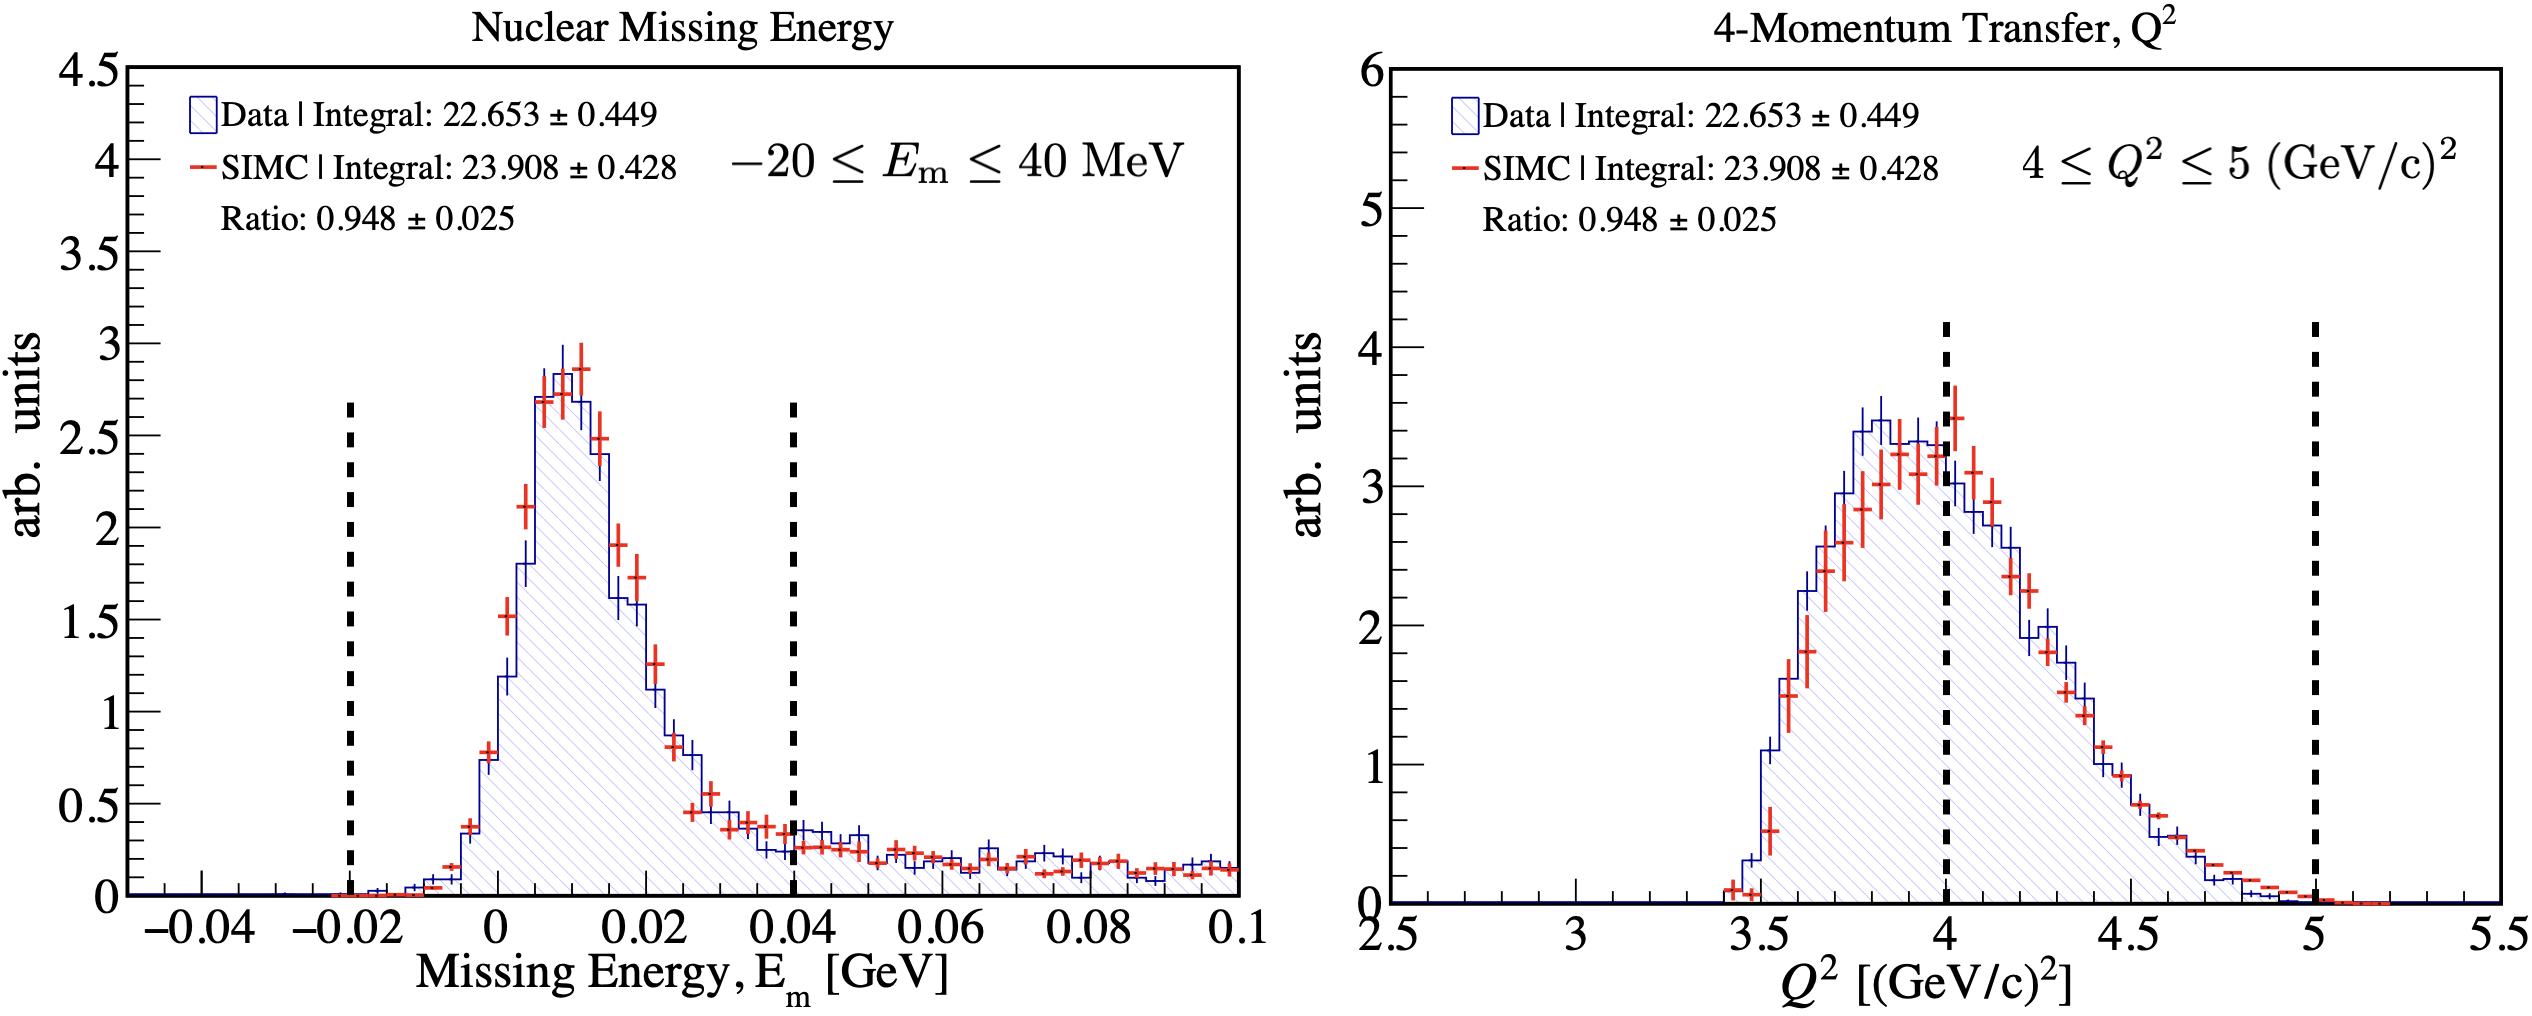
\includegraphics[scale=0.33]{Em_and_Q2_CUT_80MeV_35deg.png}
\caption{Event selection cuts on missing energy (left) and 4-momentum transfer (right).}
\label{fig:Em_Q2_cuts}
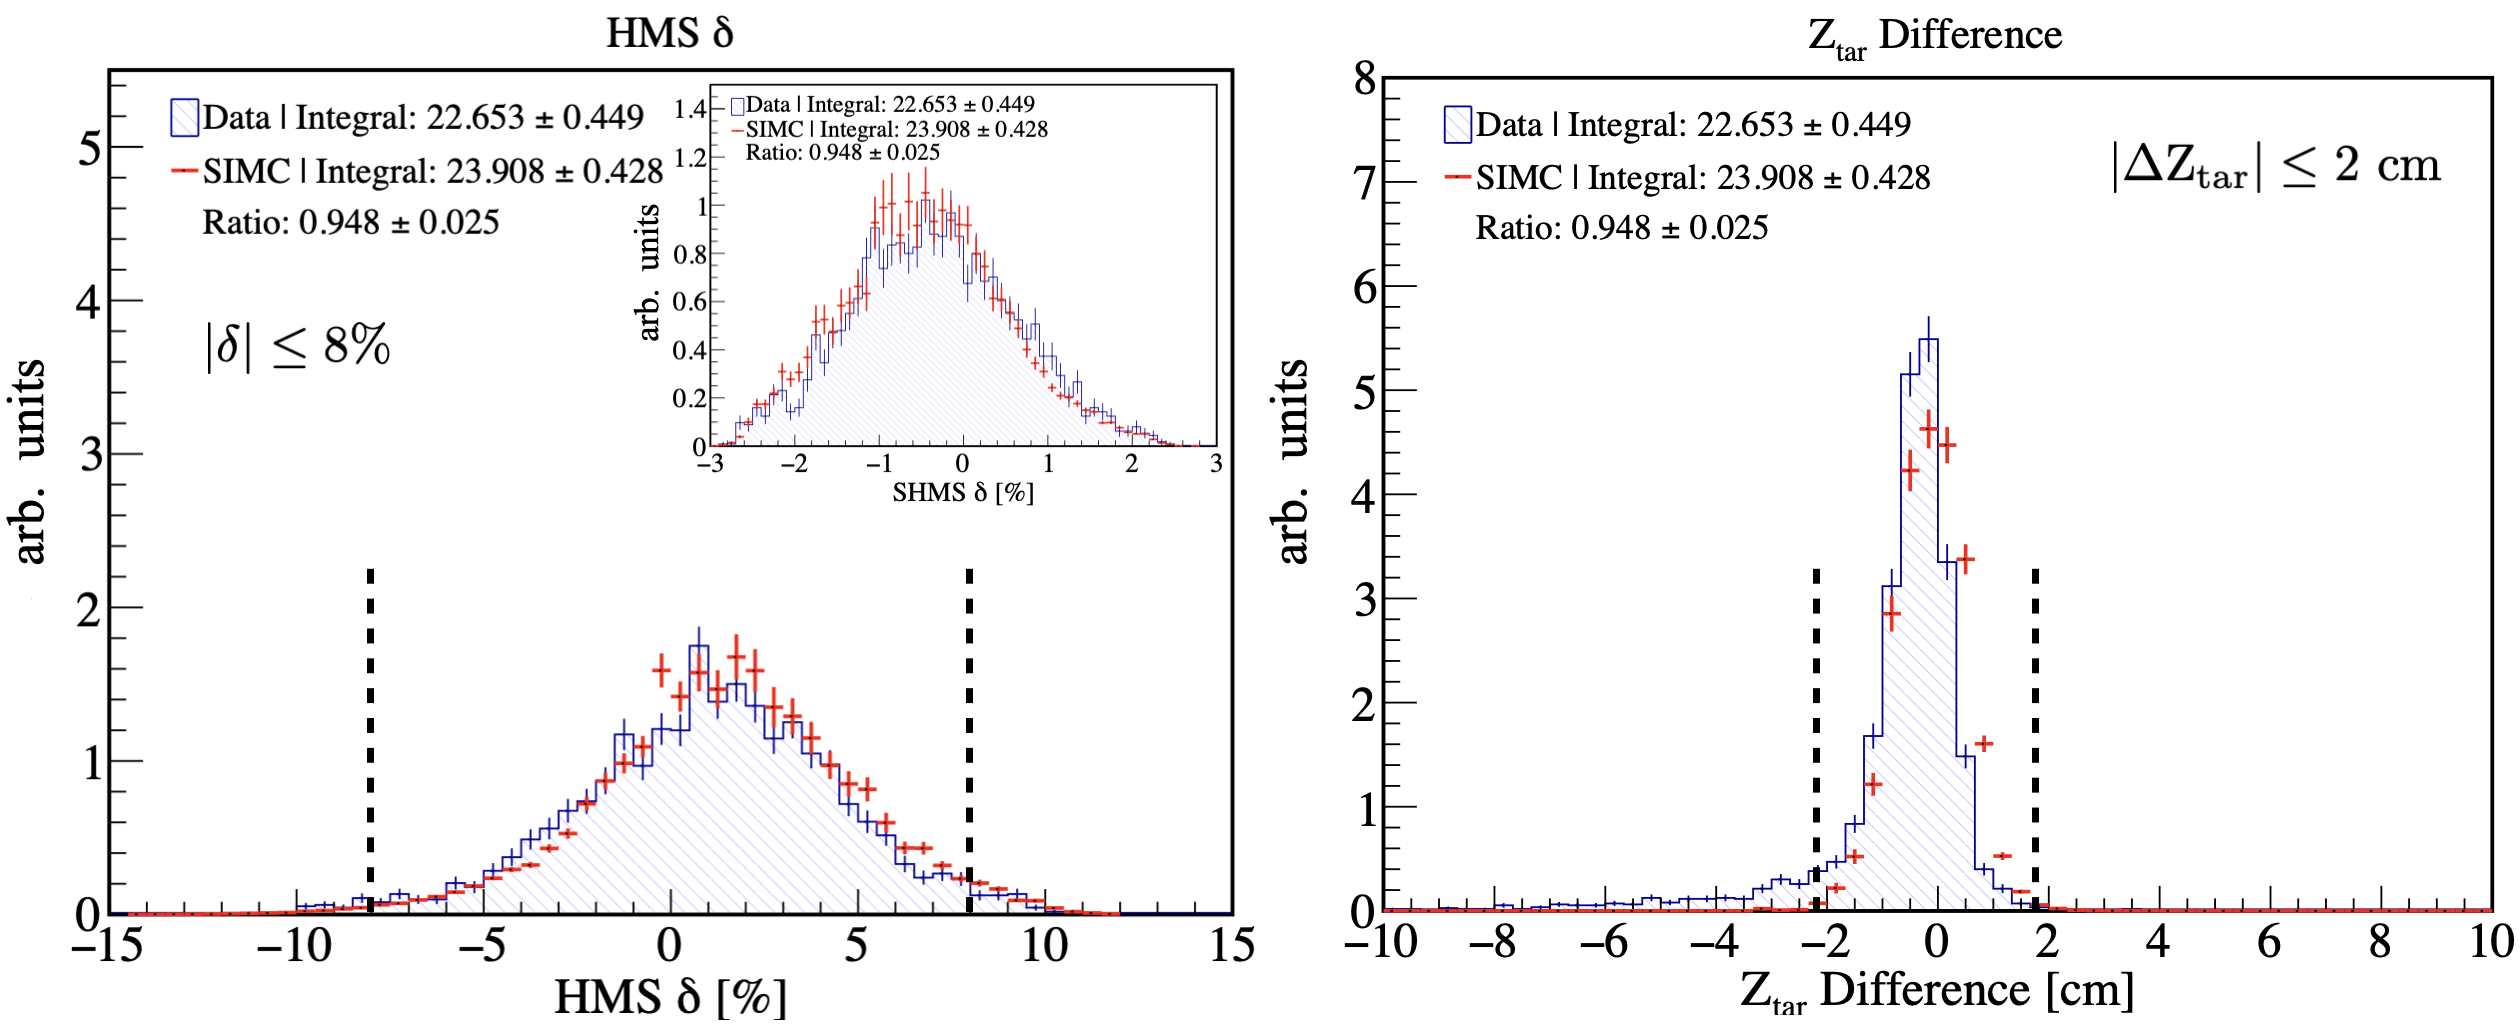
\includegraphics[scale=0.33]{deltaAcc_and_ZtarCUT_80MeV_35deg.png}
\caption{Acceptance cut on HMS momentum fraction (left) and event selection cut on the difference between the $z$-reaction vertex on both spectrometers (right).
  Inset (left): The SHMS momentum acceptance range.}
\label{fig:delta_Ztar_cuts}
\end{figure}\\
\indent Figure \ref{fig:Em_Q2_cuts} (left) shows the primary cut used to select true $^{2}\mathrm{H}(e,e'p)n$ coincidence events by requiring a missing
energy cut around the deuteron binding energy ($\sim$2.2 MeV) using the missing energy formula, $E_{\mathrm{m}} = \omega - T_{p} - T_{\mathrm{r}}$, where
$T_{p}$ is the final proton kinetic energy and $T_{\mathrm{r}}$ is the recoil particle kinetic energy which is calculated from the electron and proton
4-momentum vectors assuming an exclusive three-body final state with a recoiling neutron. The peak is not exactly at the deuteron binding energy because
energy loss corrections have not been applied to the data nor SIMC. \\
\indent Figure \ref{fig:Em_Q2_cuts} (right) shows a
kinematical cut made on the 4-momentum transfer at $Q^{2} = 4.5\pm0.5$ (GeV/c)$^{2}$
to select events only at the highest possible momentum transfers to further suppress MEC and IC. \\
\indent Figure \ref{fig:delta_Ztar_cuts} (left) shows a momentum acceptance ($\delta$) cut made on the HMS in the range $-8\%\leq\delta\leq8\%$, where the optics reconstruction
is reliable and well understood from previous experiments in the 6 GeV era. The inset shows the SHMS momentum acceptance which was constrained by that of the HMS to be
$|\delta|\lesssim$3$\%$ which is well within the reliable SHMS momentum acceptance range of $-10 \leq \delta \leq22 \%$. \\
\indent Figure \ref{fig:delta_Ztar_cuts} (right) shows a reaction vertex cut
on the difference between the HMS and SHMS reconstructed reaction vertices along the $z$-coordinate (target length). The cut is made at $\pm2$ cm relative to the histogram peak.
If the events originated from the same reaction vertex (i.e., true coincidences), the difference should peak at zero with a finite resolution width. If the events are uncorrelated
(i.e., accidental coincidences), however, the reconstruction along the $z_{\mathrm{v}}$-vertex can vary significantly between the two spectrometers, which contribute to the tails of the
distribution.\\
\begin{figure}[!h]
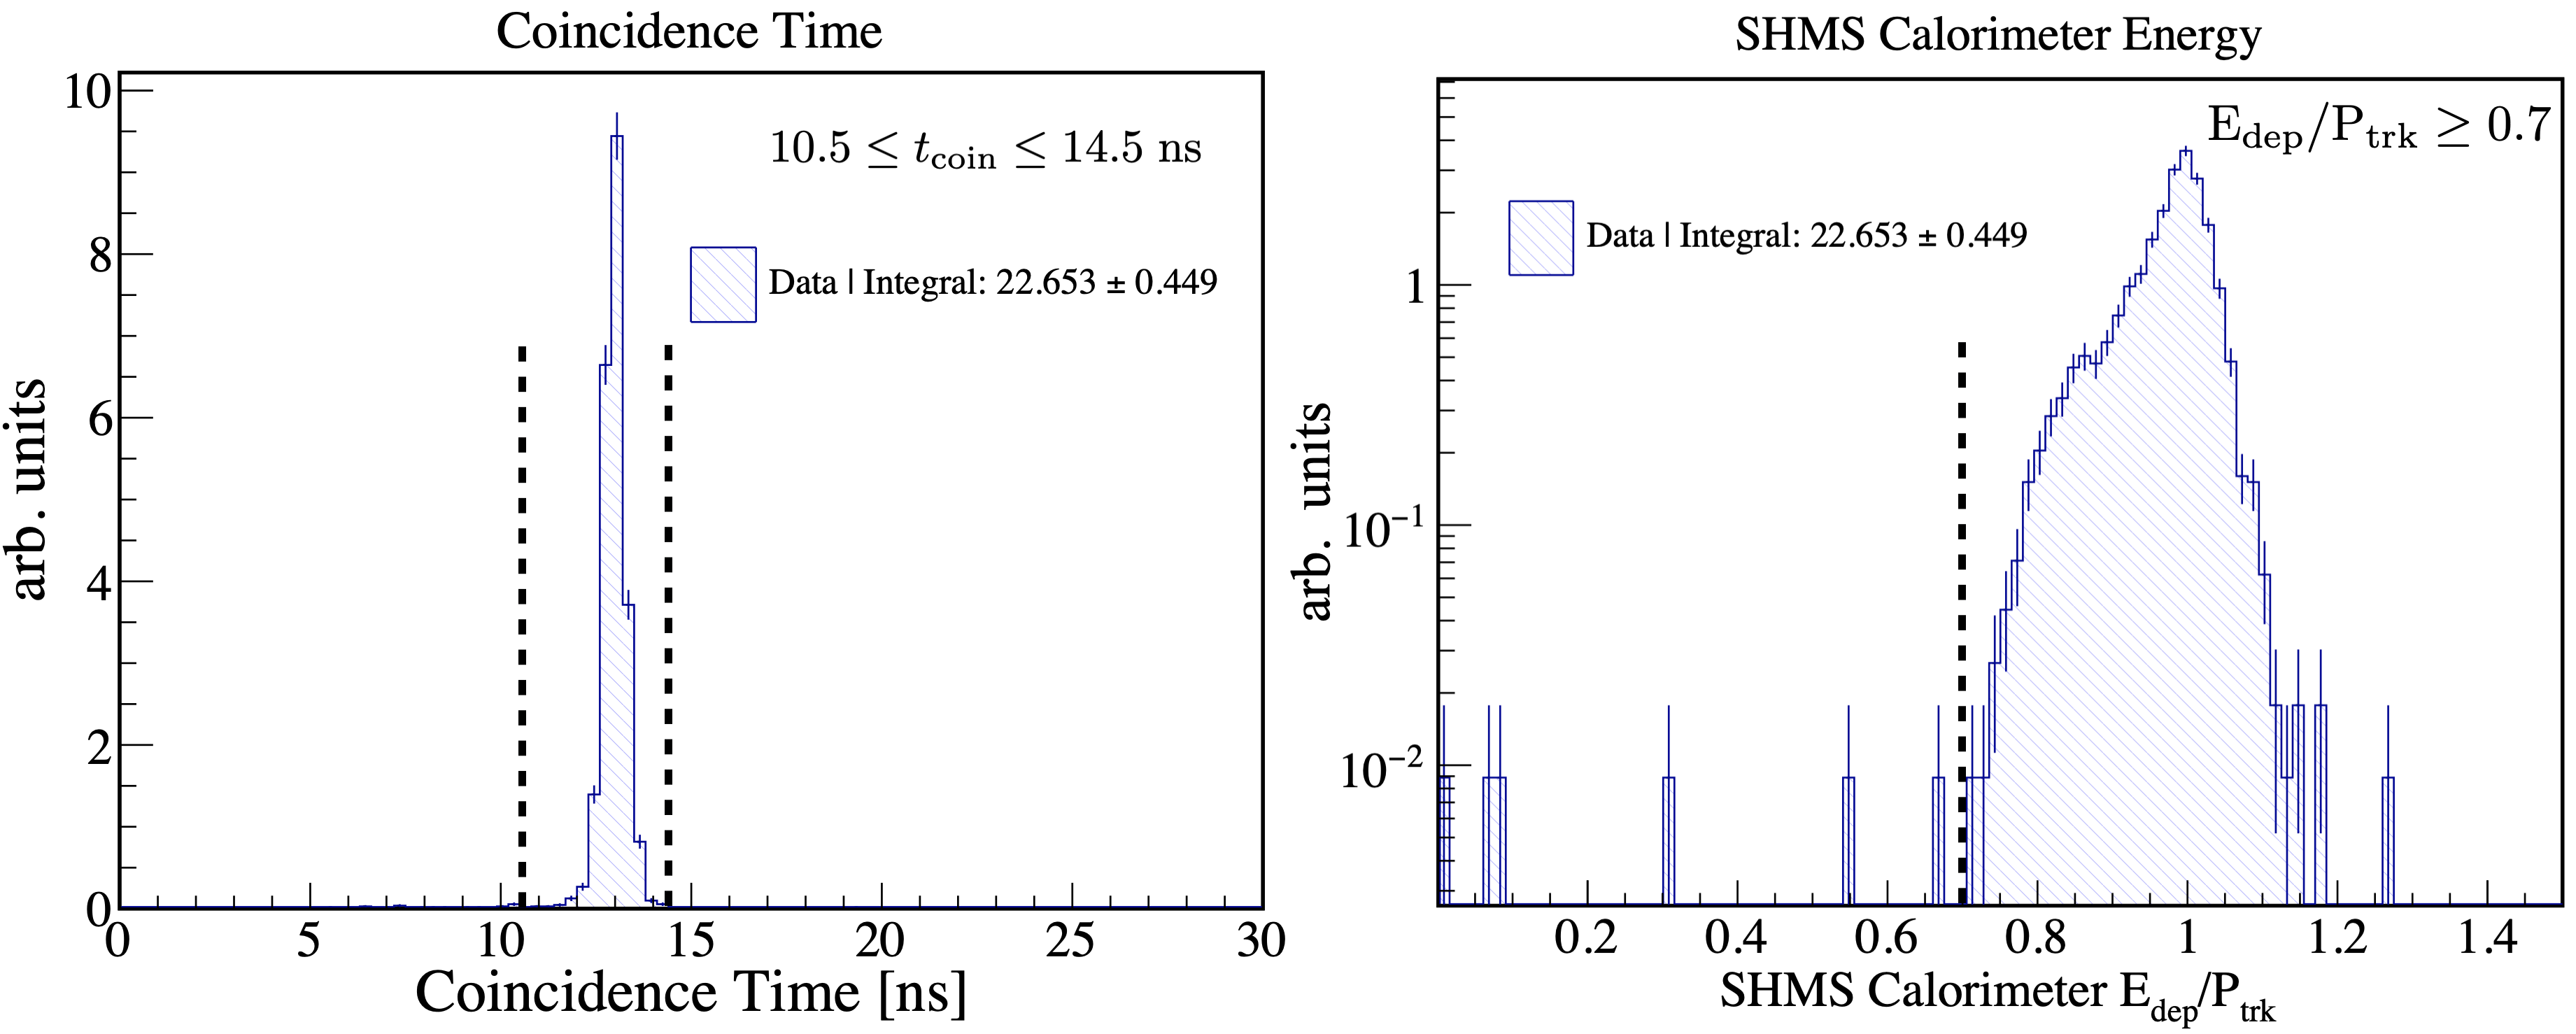
\includegraphics[scale=0.23]{coin_and_eCal_CUT_80MeV_35deg.png}
\caption{Event selection cuts on the electron-proton ($ep$) coincidence time (left) and total deposited energy on calorimeted normalized by the particle track momentum (right).}
\label{fig:coin_ecal_cuts}
\end{figure}\\
\indent Figure \ref{fig:coin_ecal_cuts} (left) shows a coincidence time cut on the $ep$ coincidence time spectrum formed by requiring a logic signal of
at least 3 out of 4 scintillator planes between both spectrometers. The spectrum is very clean as the typical 4 ns beam bunch structure due to accidental
coincidences is not observed. \\
\indent Figure \ref{fig:coin_ecal_cuts} (right) shows a particle identification cut on the SHMS calorimeter total energy
deposited normalized by the particle track momentum. This cut was used to separate electrons from background (pions), however, the spectrum shows a very clean distribution
with a peak at about one indicating the detected particles were electrons.
\begin{figure}[!h]
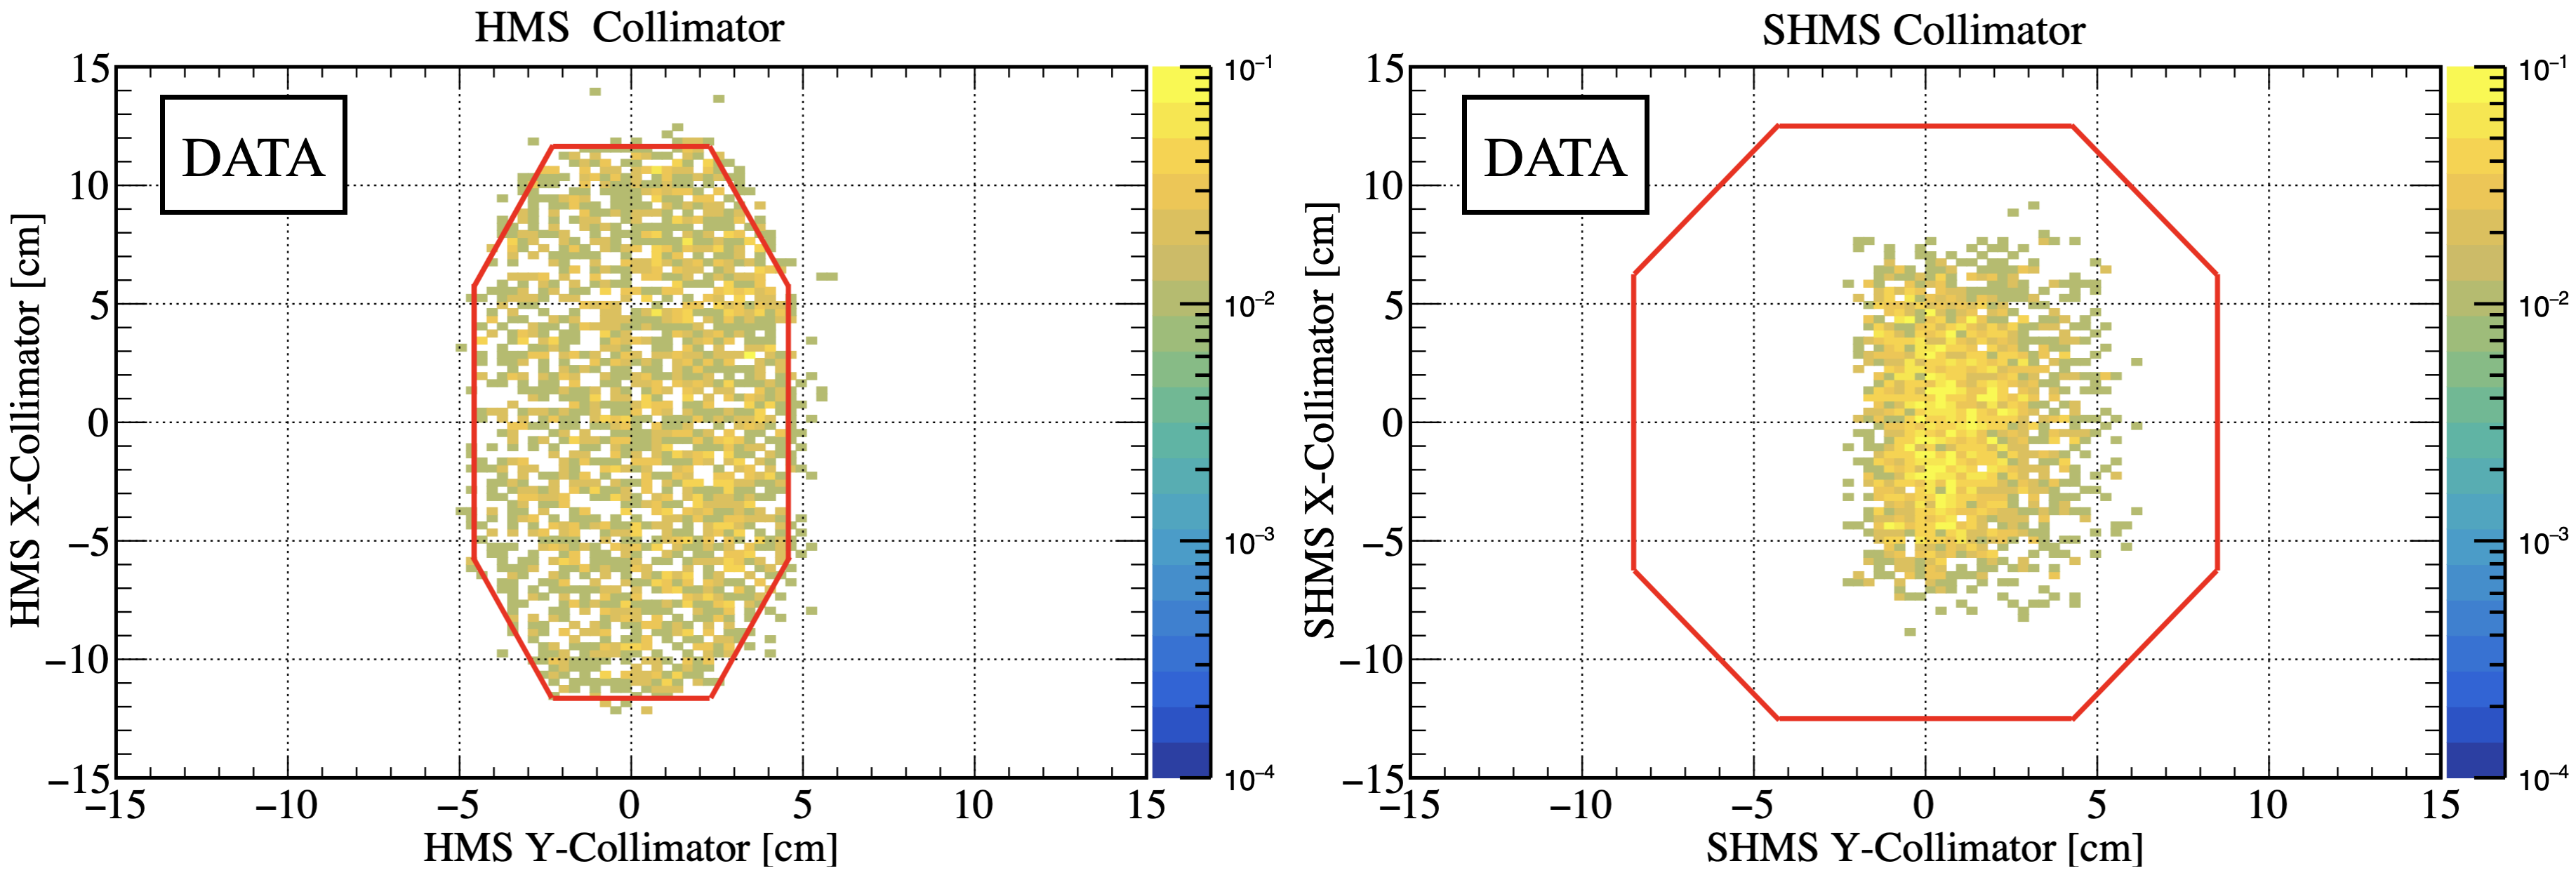
\includegraphics[scale=0.24]{collimator_CUT_80MeV_35deg_data.png}
\caption{(left) Geometrical acceptance cut on reconstructed events projected at the HMS collimator. (right) The SHMS events (correlated with HMS events on left plot),
  projected at the SHMS collimator. The $z$-axis (color palette) is in arbitrary units.}
\label{fig:data_coll_cuts}
\end{figure}
\clearpage
\indent Figure \ref{fig:data_coll_cuts} (left) shows a geometrical (red octogon) cut on the reconstructed events projected at the HMS collimator to ensure
that all events that enter the spectrometer pass through the collimator, and not re-scatter at the edges. This cut is needed since protons that enter the
HMS can punch through the collimator with a probability that is related to the proton-Tungsten total cross section.\\
\indent Figure \ref{fig:data_coll_cuts} (right)
shows the correlated events projected at the SHMS collimator which clearly shows that the events are well within the collimator which indicates that the SHMS
acceptance is driven by that of the HMS. Figure \ref{fig:simc_coll_cuts} shows the same acceptance cuts as previously described, but for simulation. The colored
$z$-axis in both figures is given in arbitrary units.\\
\begin{figure}[!h]
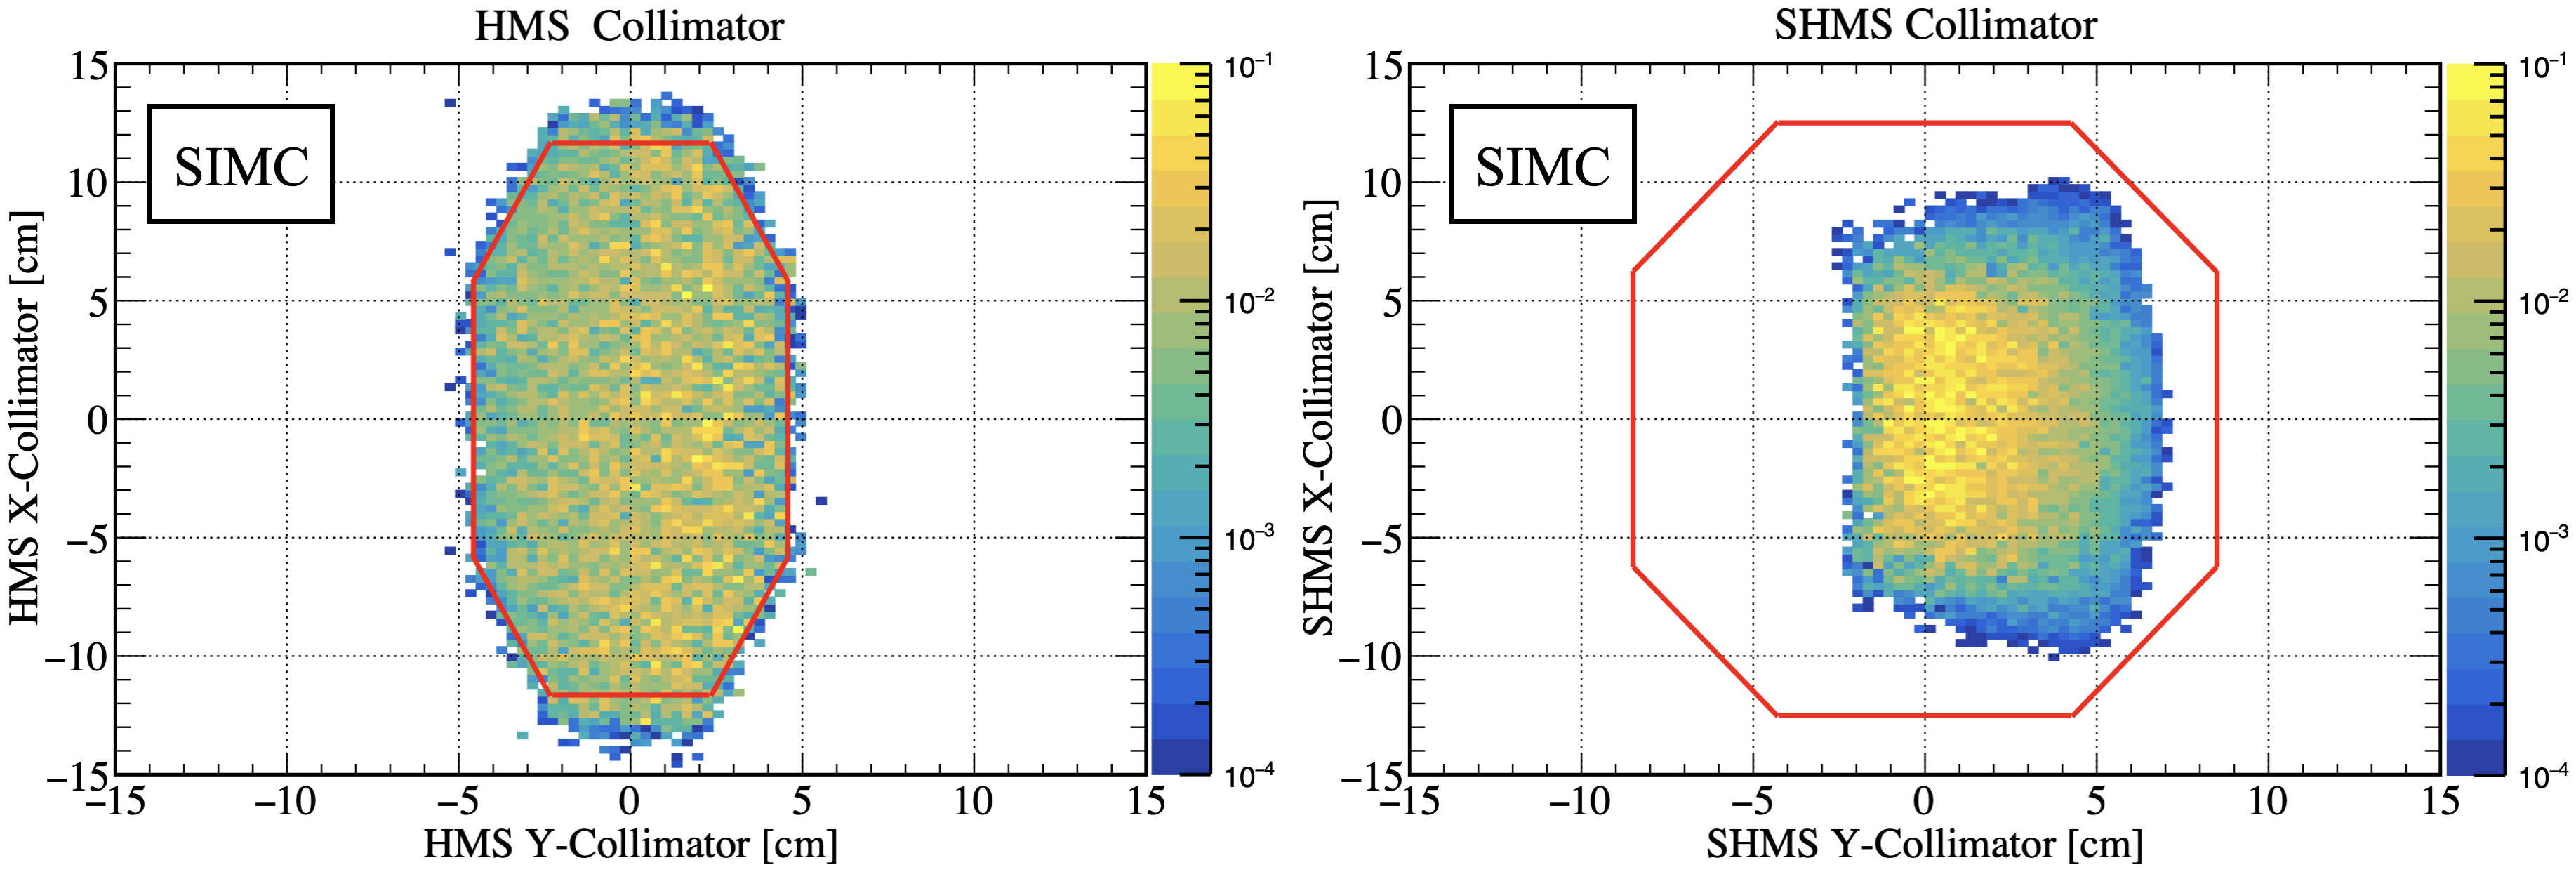
\includegraphics[scale=0.25]{collimator_CUT_80MeV_35deg_SIMC.png}
\caption{Same as Fig. \ref{fig:data_coll_cuts}, but for simulation.  The $z$-axis (color palette) is in arbitrary units.}
\label{fig:simc_coll_cuts}
\end{figure}
\section{\large Deuteron Kinematic Distributions }
\indent Figures \ref{fig:d2_kin_35deg} and \ref{fig:d2_kin_45deg} show the fundamental kinematic variable distributions for each of the
central missing momentum settings at $\theta_{nq}=35^{\circ}$ and $45^{\circ}$. The data has been normalized by the total charge and corrected
for the inefficiencies described in the Letter. The same event selection cuts mentioned in the previous section were applied. 
\begin{figure}[!h]
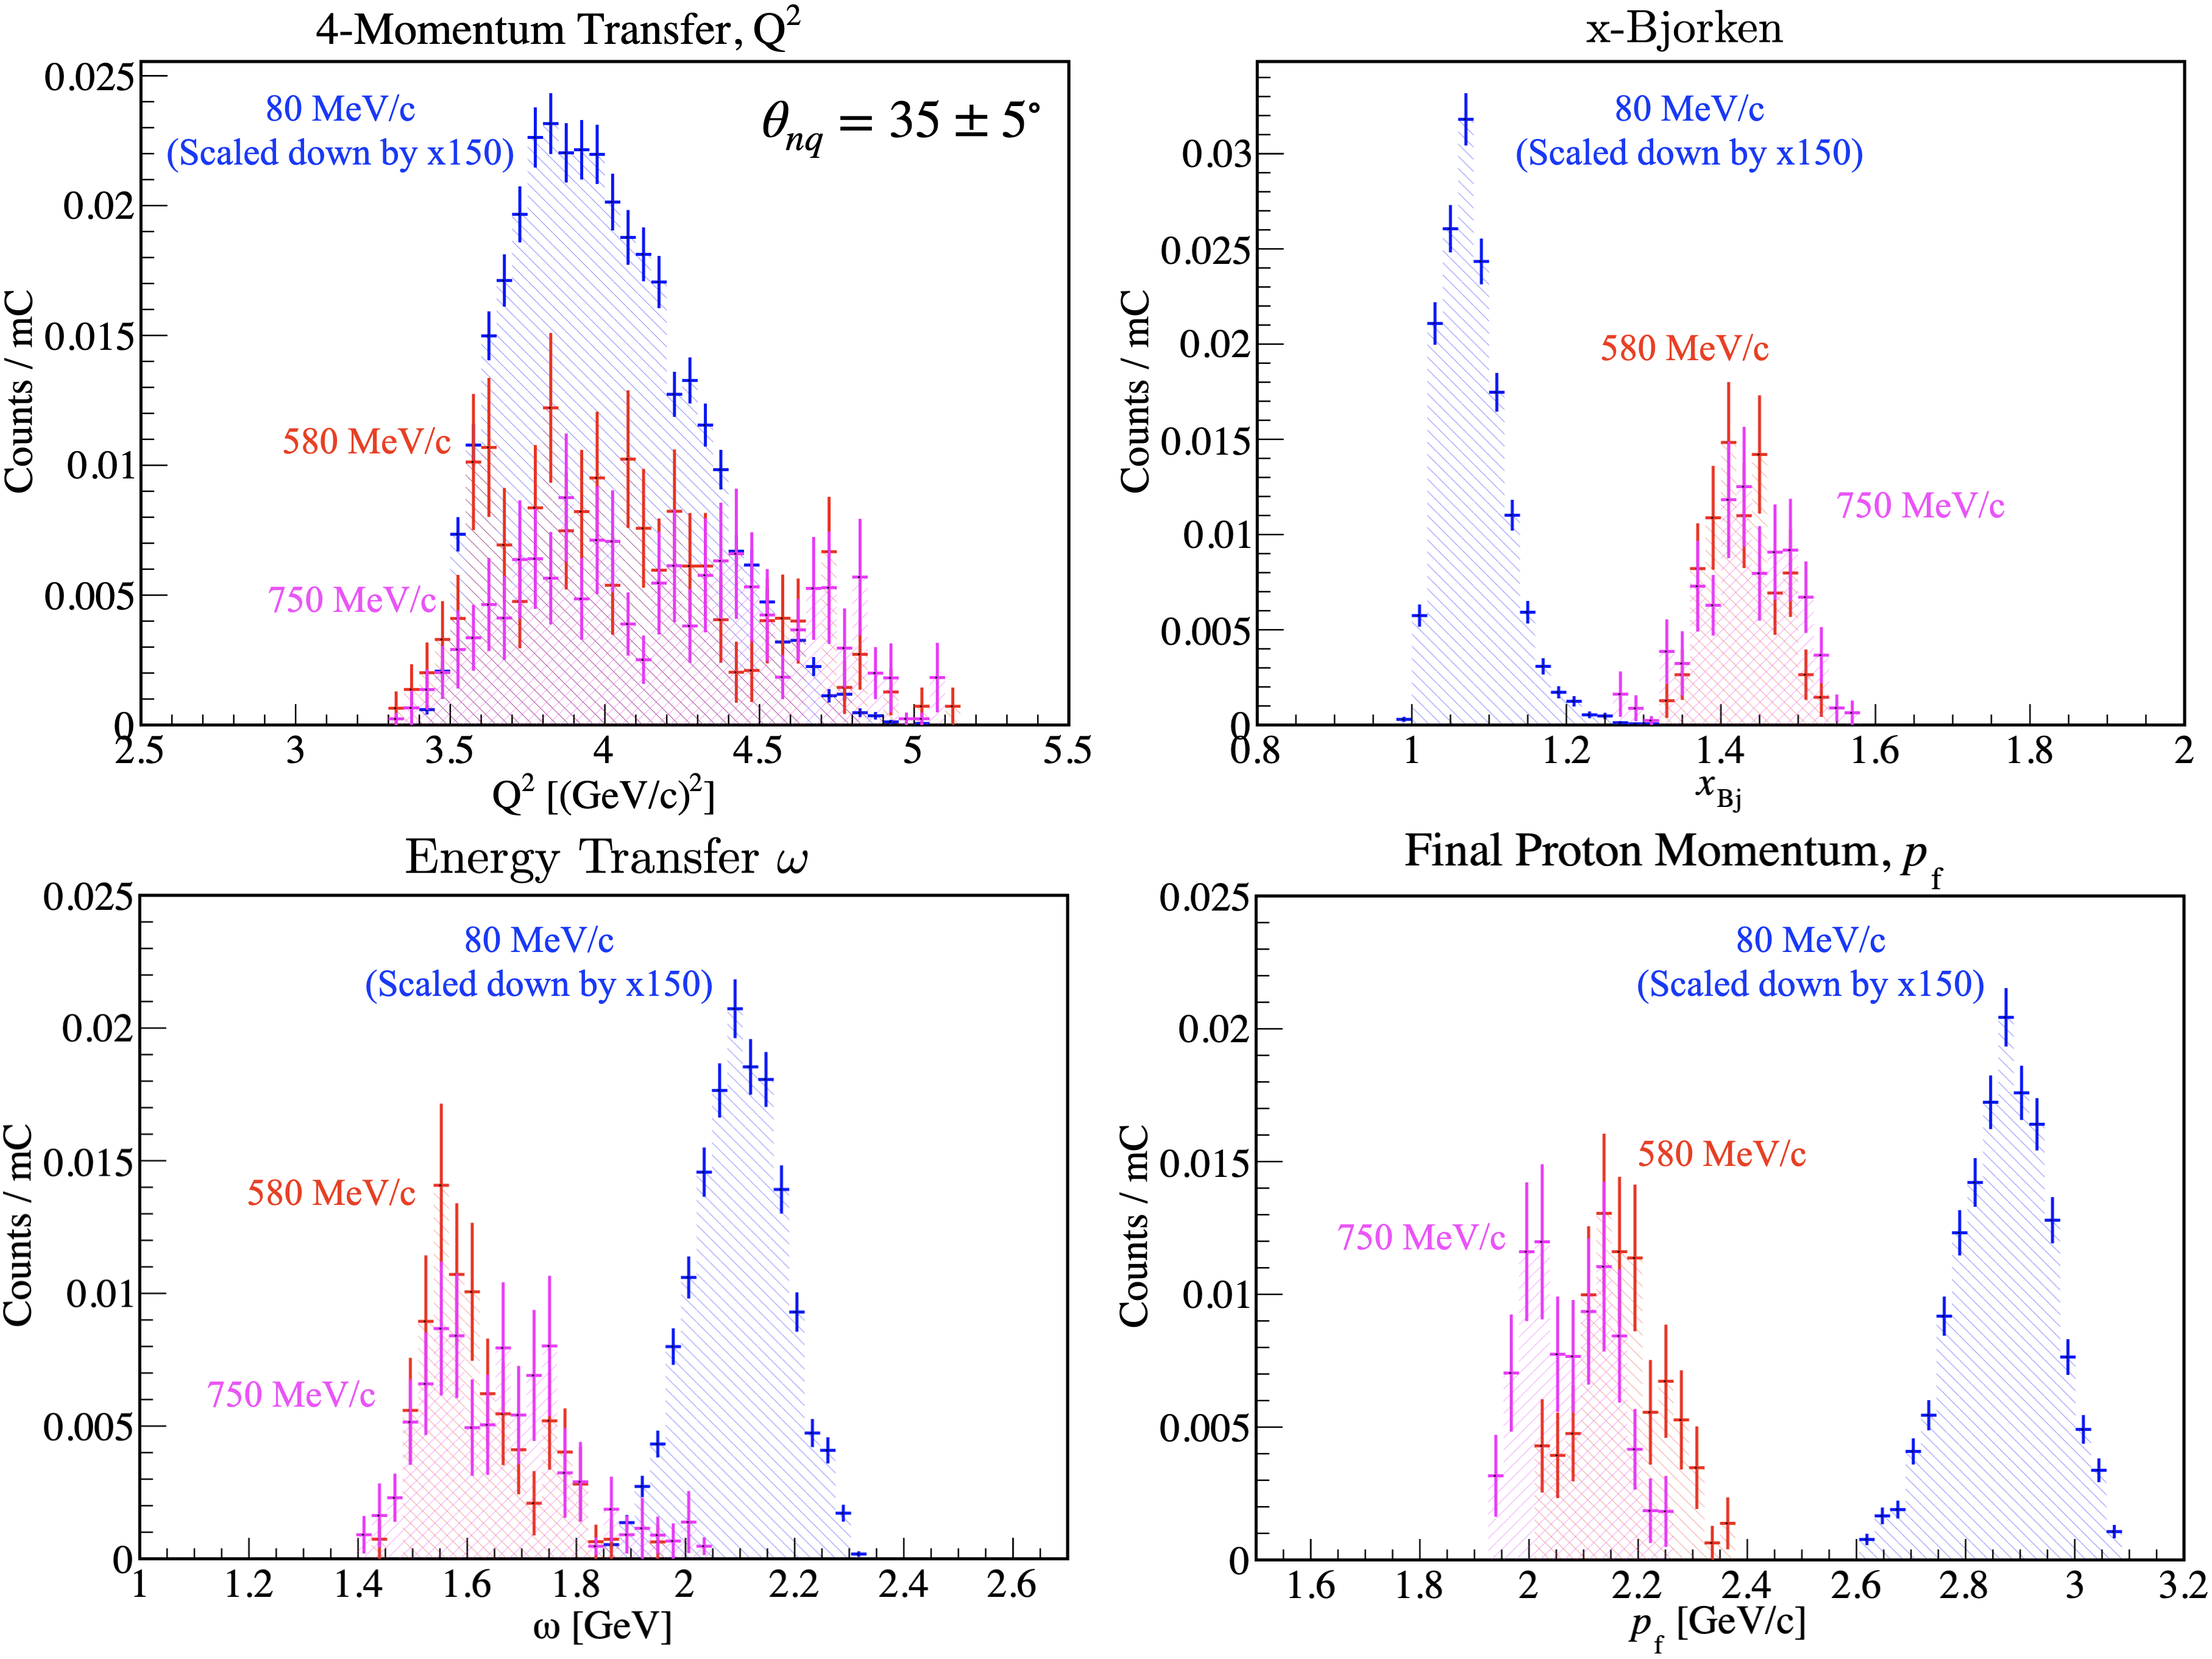
\includegraphics[scale=0.17]{d2_kin_thnq35.png}
\caption{Deuteron kinematic distributions for the 80 (blue), 580 (red) and 750 (magenta) MeV/c setting at $\theta_{nq}=35^{\circ}$.}
\label{fig:d2_kin_35deg}
\end{figure}
\begin{figure}[!h]
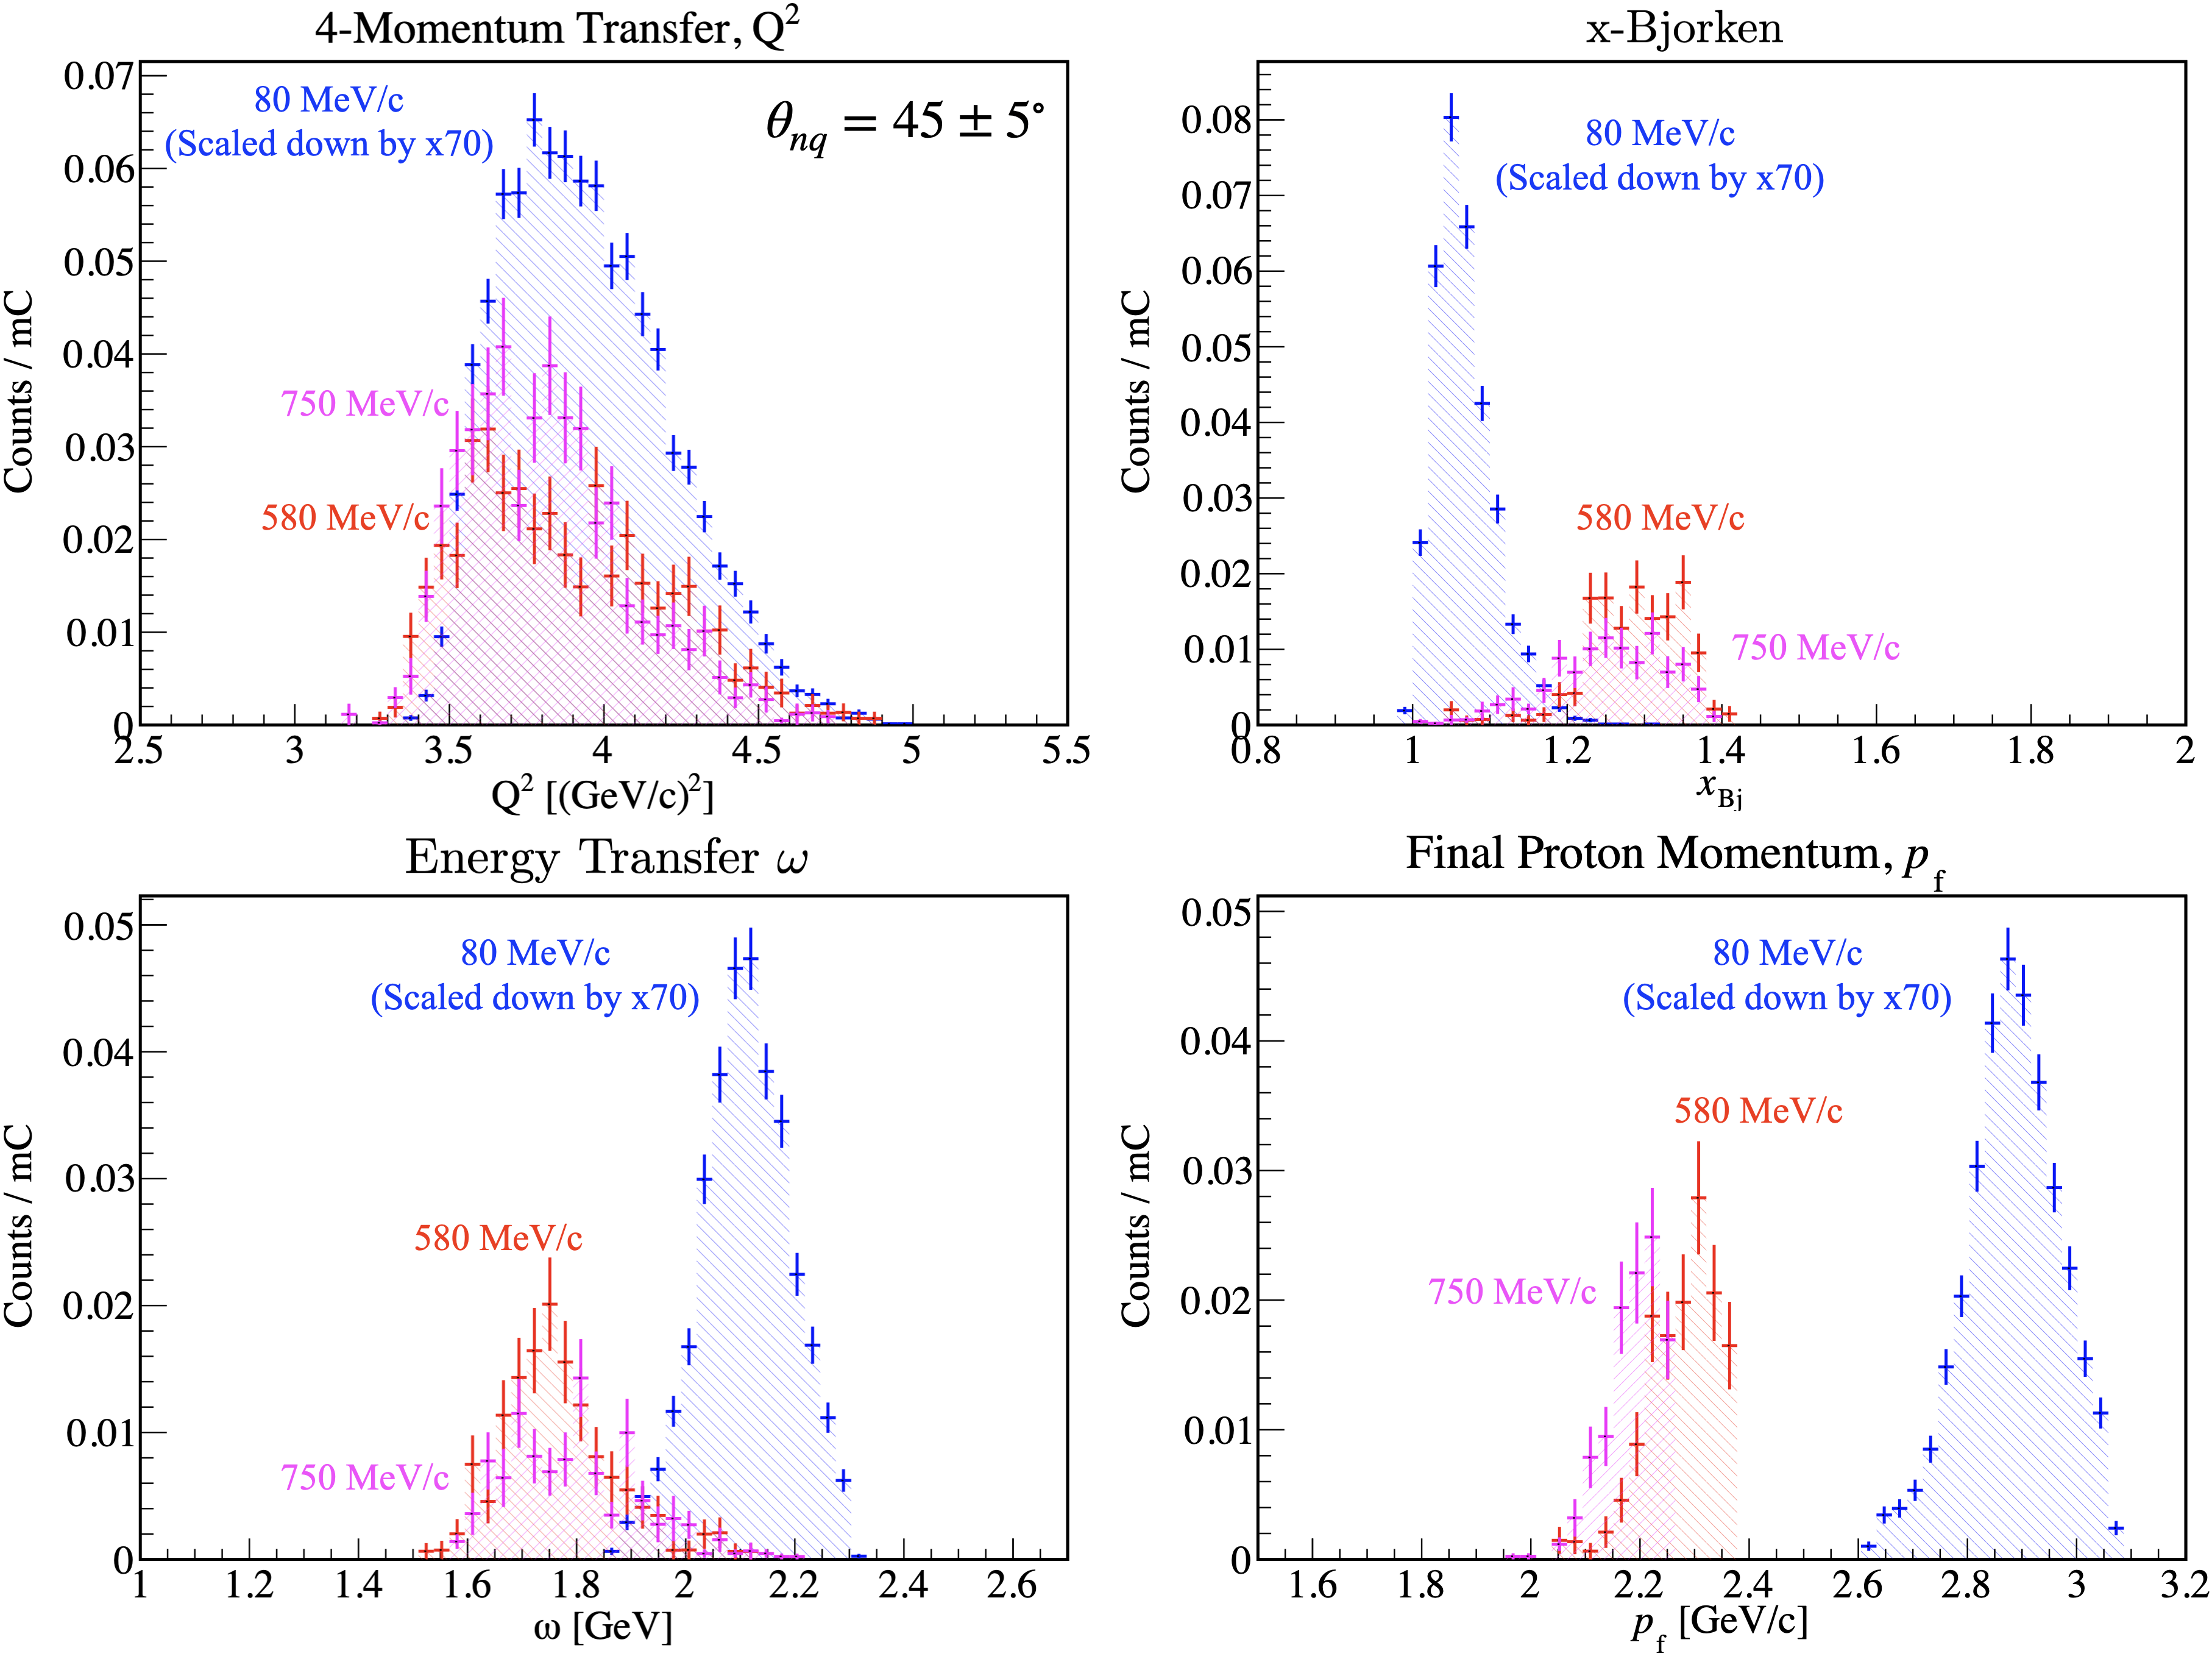
\includegraphics[scale=0.17]{d2_kin_thnq45.png}
\caption{Same as Fig. \ref{fig:d2_kin_35deg}, but for $\theta_{nq}=45^{\circ}$}
\label{fig:d2_kin_45deg}
\end{figure}
\section{\large Estimate of the Target Cell Endcaps Contribution to the Data Yield}
\indent To estimate the contribution to the yield due to the electron interaction with the aluminum endcaps of the target cell,
a sample of events were selected in the negative part of the missing energy spectrum using the deuteron high missing momentum settings (580 and 750 MeV/c).
We assume that the contribution due to the target endcaps is constant across the missing energy spectrum, therefore, by selecting a sample in the
negative part of the spectrum over a specific range, we can estimate the endcaps contribution beneath the deuteron missing energy peak over the same range.\\
\indent Figure \ref{fig:tgt_wall} shows the missing energy spectrum for the 580 MeV/c setting (left) and the corresponding reconstructed SHMS $z$-vertex (right) for the specified
range. The integral over endcaps and $^{2}\mathrm{H}(e,e'p)n$ events show that the contribution from the cell walls has an upper limit of 0.00806/0.275 $\sim$ 0.0293 or approximately 2.9 $\%$
as the integral was done over all recoil angles, $\theta_{nq}$. This result was added quadratically to the overall normalization error.
\begin{figure}[!h]
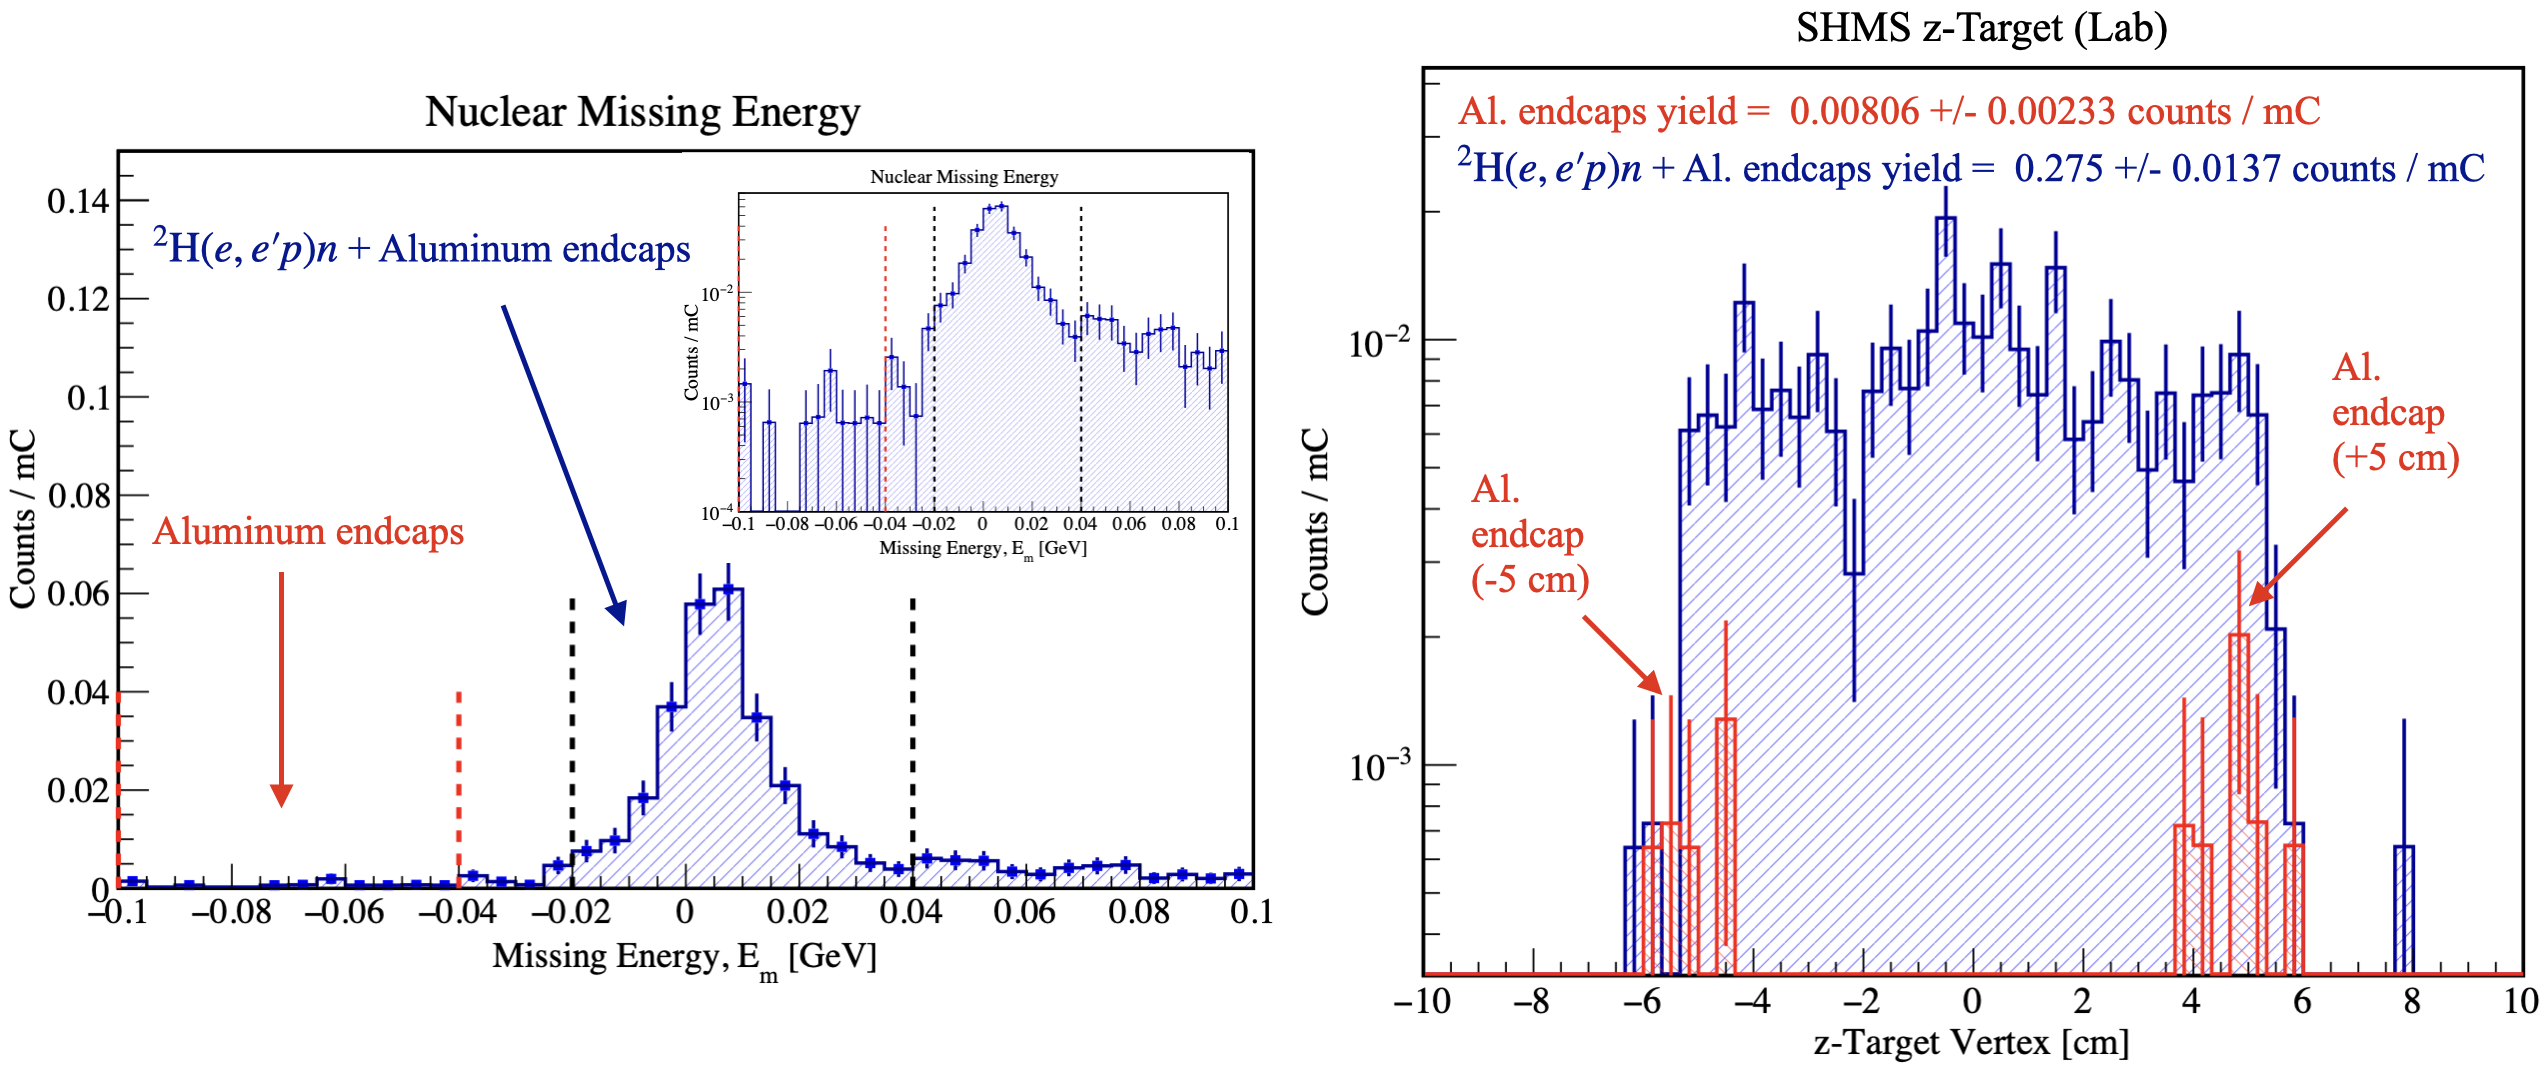
\includegraphics[scale=0.33]{tgt_bkg_d2_pm580_allthnq.png}
\caption{(left) Missing energy spectrum for the deuteron 580 MeV/c setting with event selection region corresponding to Aluminum endcaps (in red) and deuteron missing energy peak over
  a 60 MeV range, each.  Inset (left): Missing energy spectrum on a logarithmic scale. (right) The SHMS $z$-reaction vertex corresponding to
  the specified region in the missing energy spectrum.}
\label{fig:tgt_wall}
\end{figure}
\section{\large Cross-Section Extraction}
\indent The average experimental cross section was extracted by taking the ratio of the radiative corrected data yield ($Y_{\mathrm{corr}}$) to the Monte Carlo generated phase space volume for each
kinematic bin in ($\theta_{nq}$, $p_{\mathrm{r}}$). For illustration purposes, Fig. \ref{fig:Pm_Ps} shows the experimental data yield (left) and the spectrometers' phase space volume (right) binned in
missing momentum and $\theta_{nq} = 35^{\circ}$ and  $45^{\circ}$ bins for each of the three central momentum settings. Figure \ref{fig:RedXsec_overlap} shows the reduced cross section overlap for the high
$p_{\mathrm{r}}$ region. A detailed discussion of how the experimental and reduced cross sections were extracted can be
found in Sections 5.1 and 6.1 of Ref. \cite{cyero_phdthesis}.
\begin{figure}[!h]
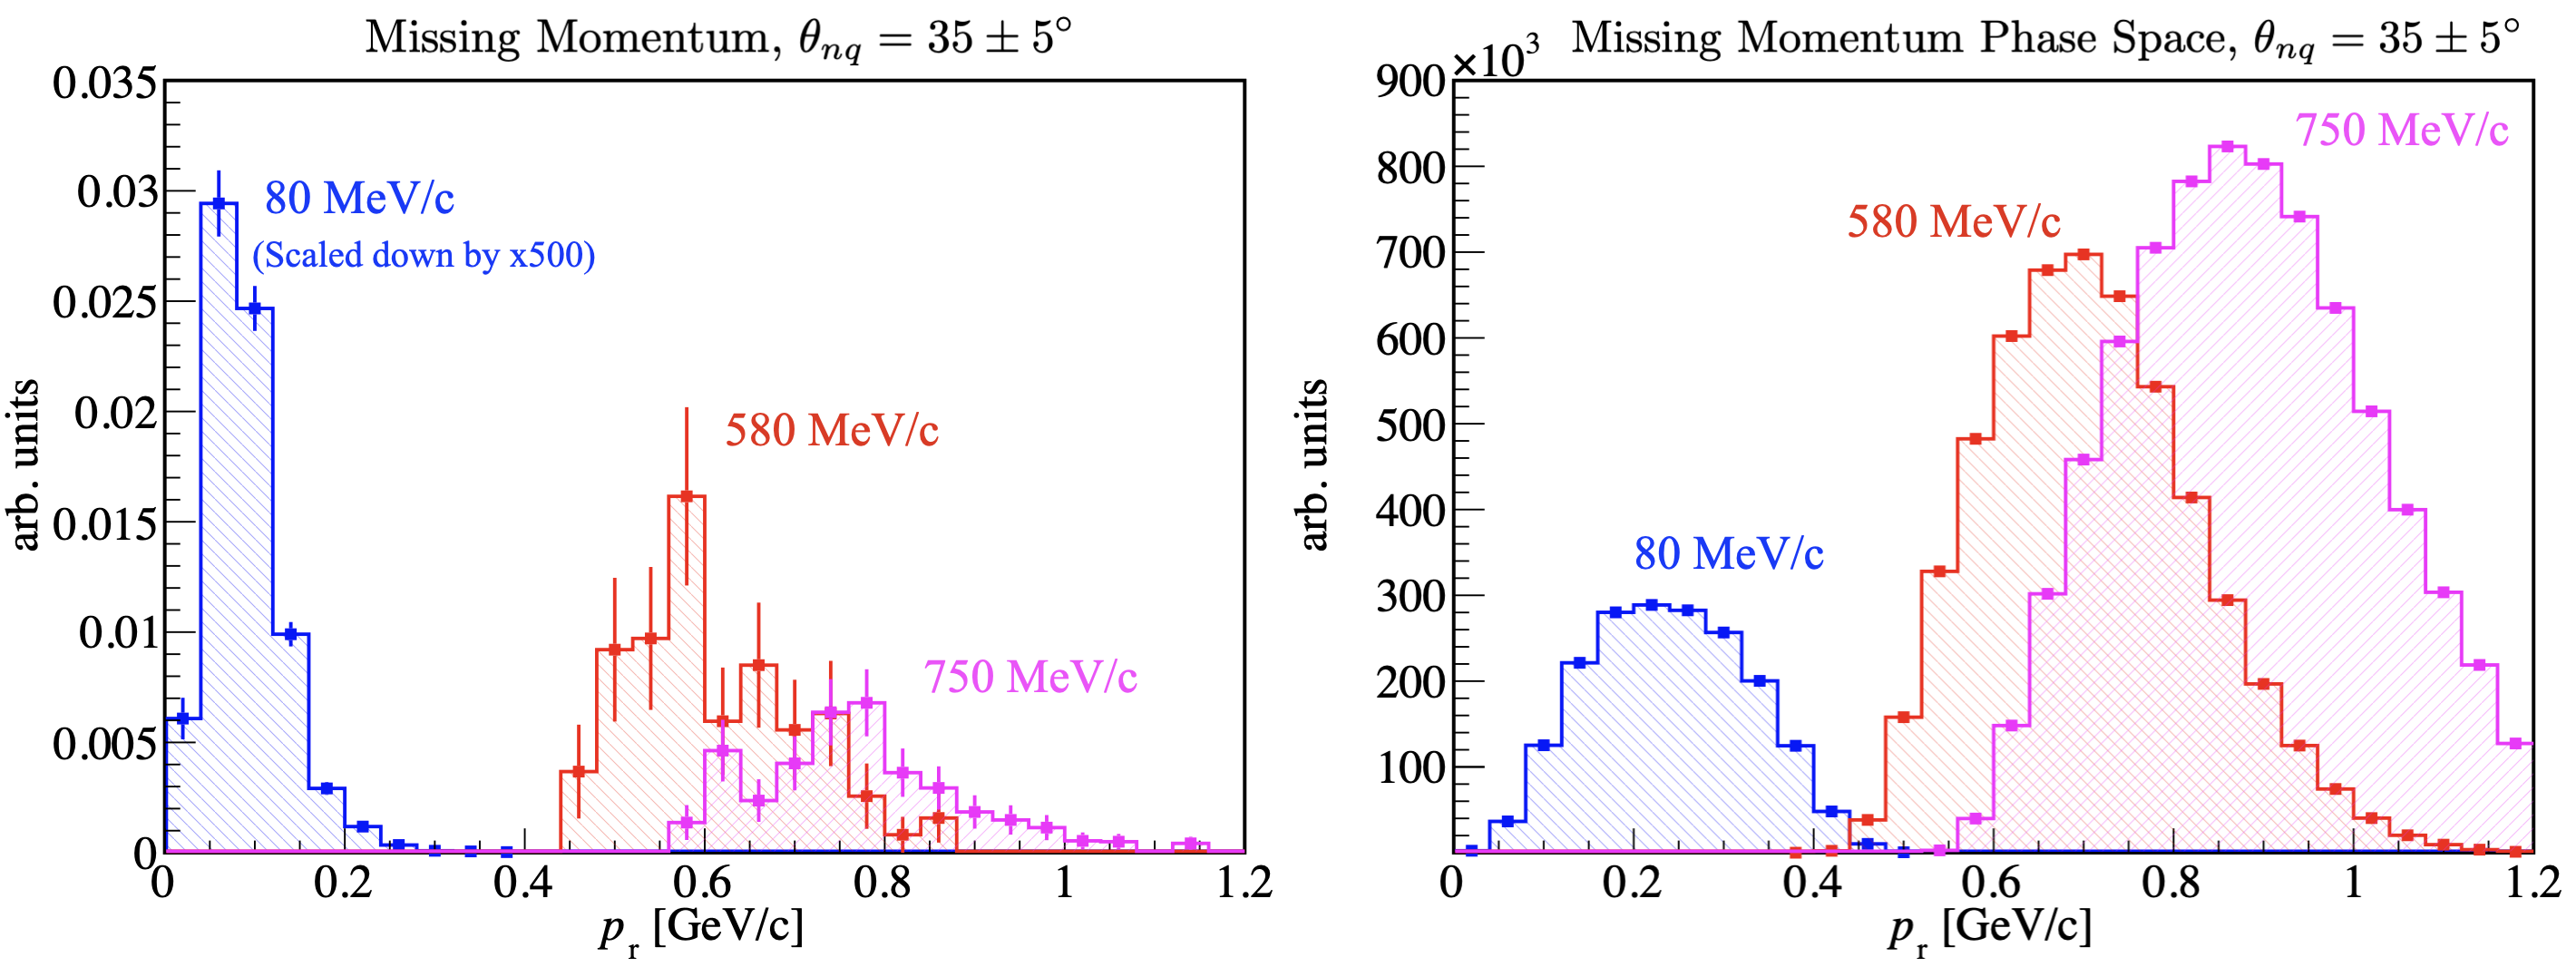
\includegraphics[scale=0.30]{Pr_and_Ps_35deg.png}
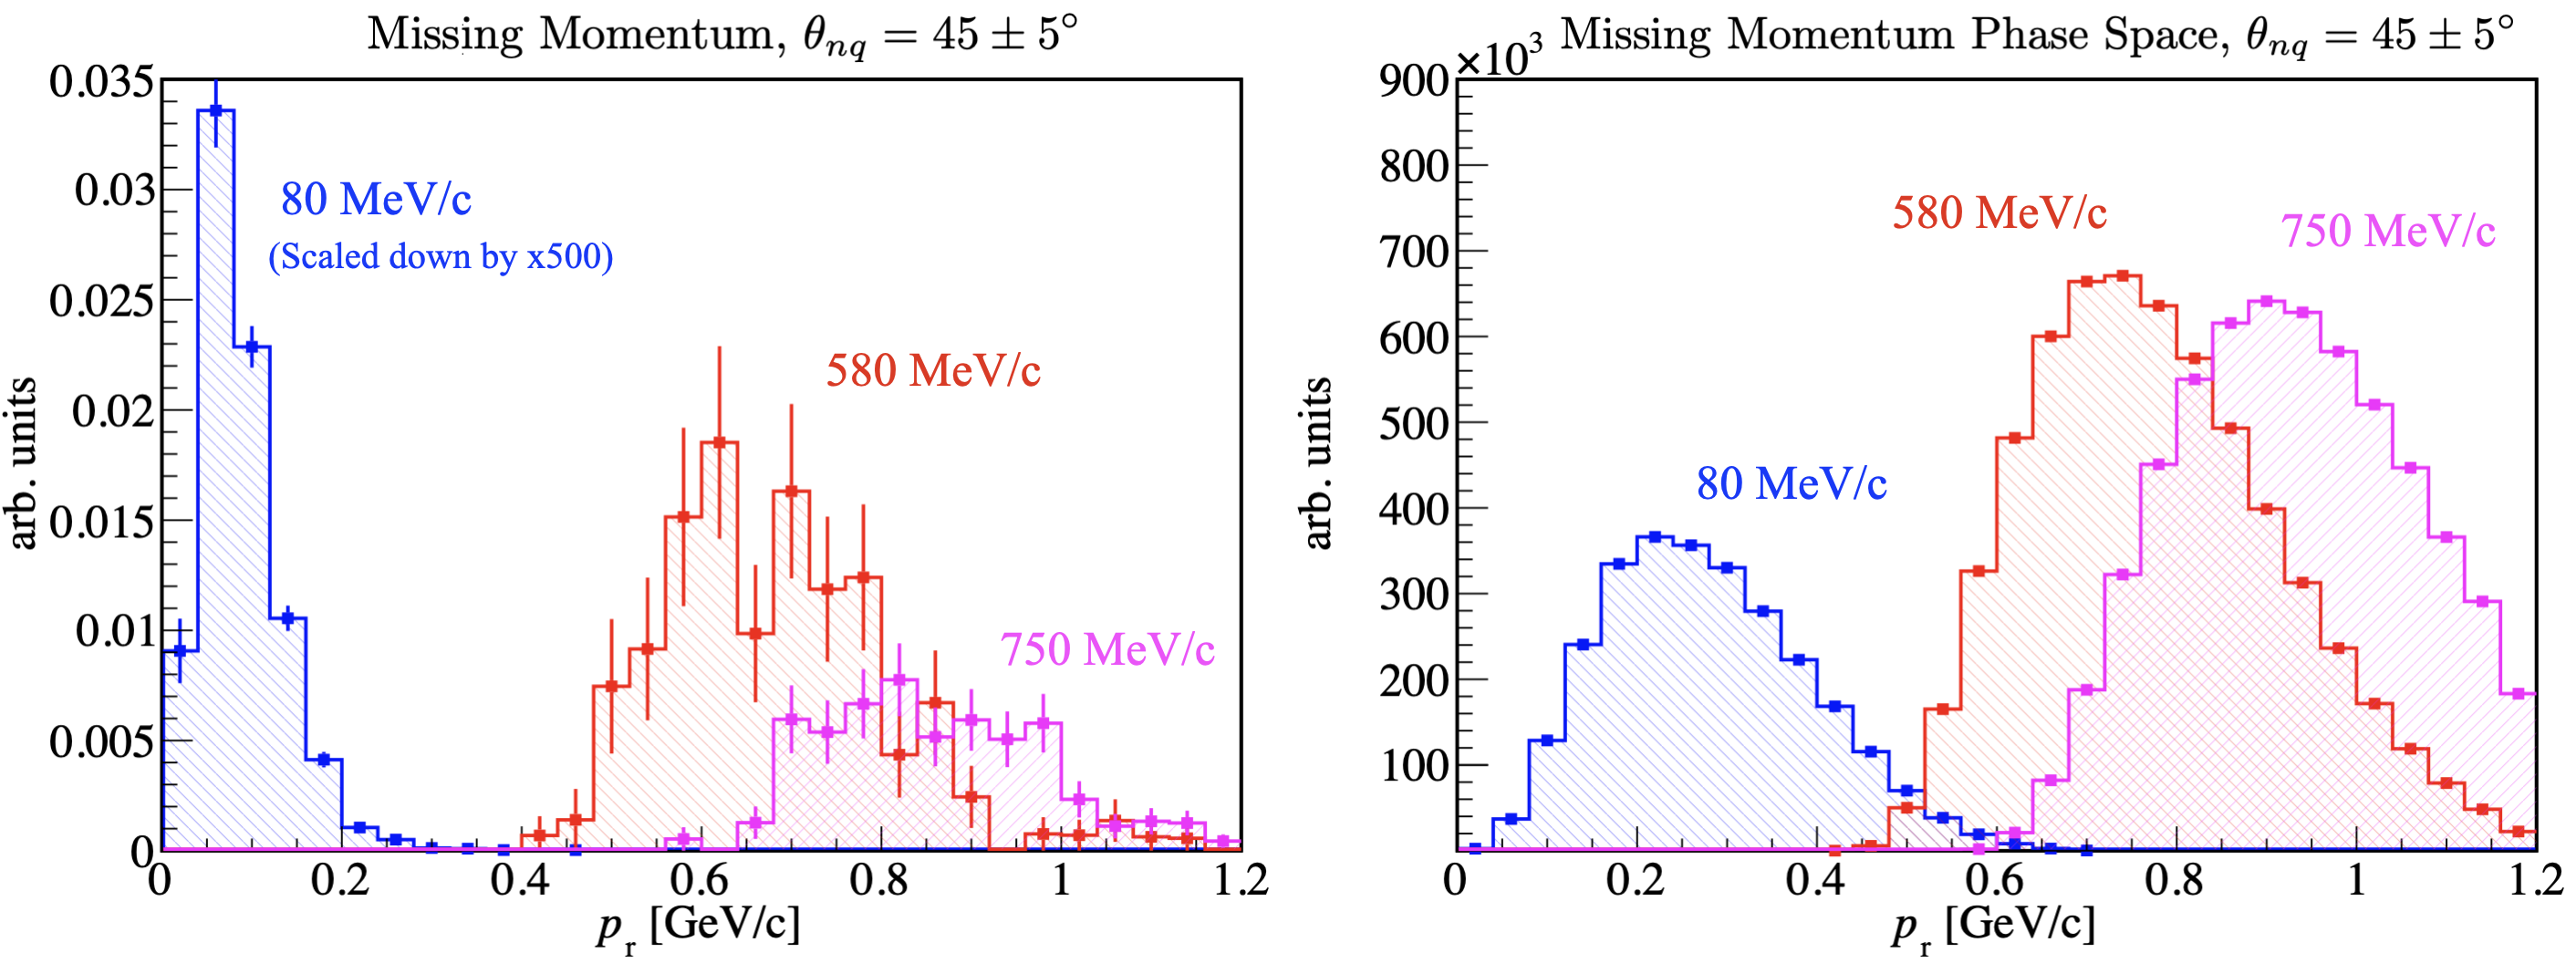
\includegraphics[scale=0.30]{Pr_and_Ps_45deg.png}
%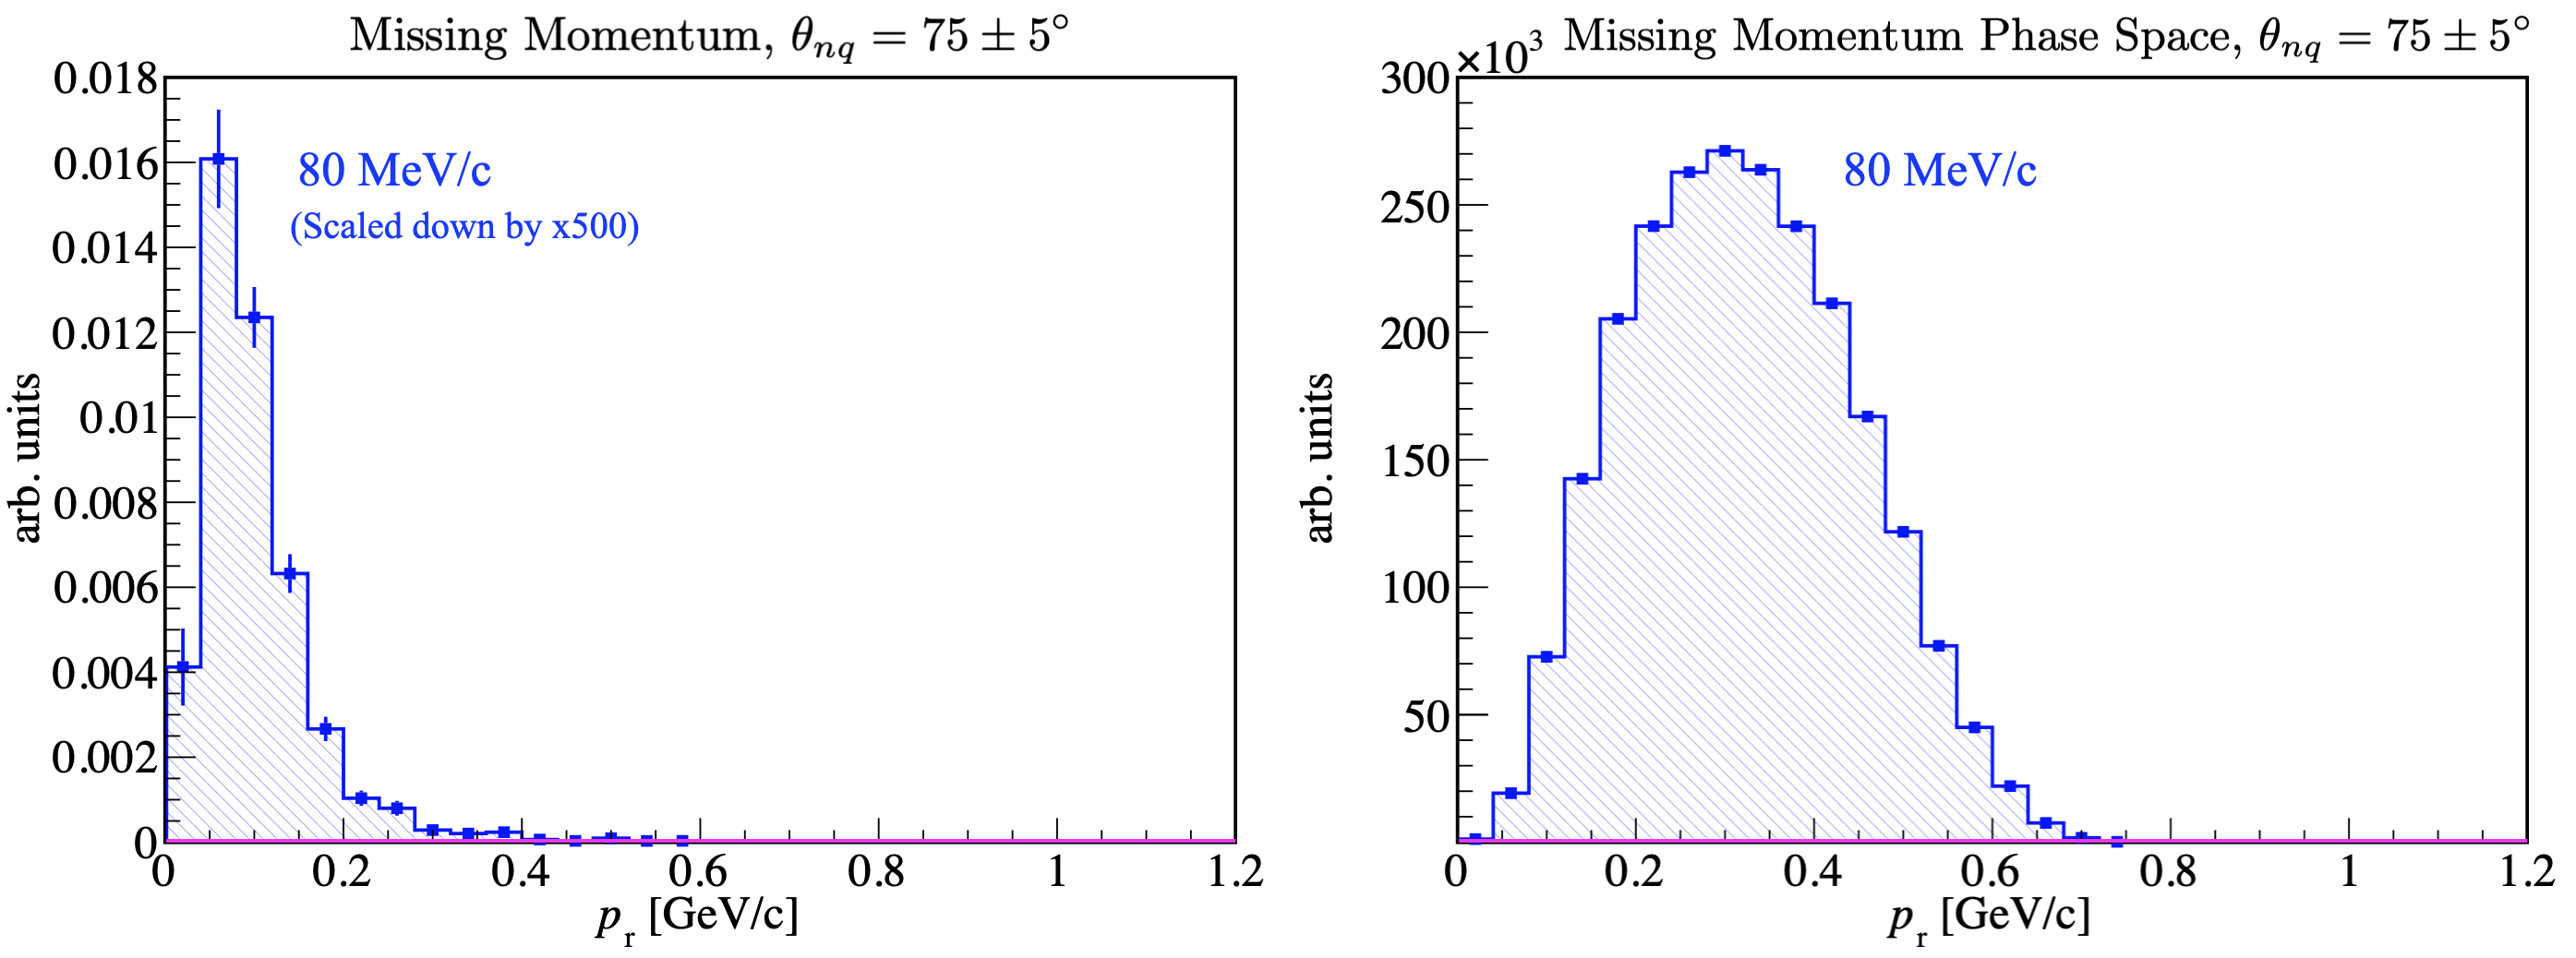
\includegraphics[scale=0.31]{Pr_and_Ps_75deg.png}
\caption{(left column) Experimental neutron recoil (``missing'') momentum distribution for each of the three central settings. (right column) Monte Carlo (un-weighted) events generated over
  the spectrometers' phase space volume binned in missing momentum.}
\label{fig:Pm_Ps}
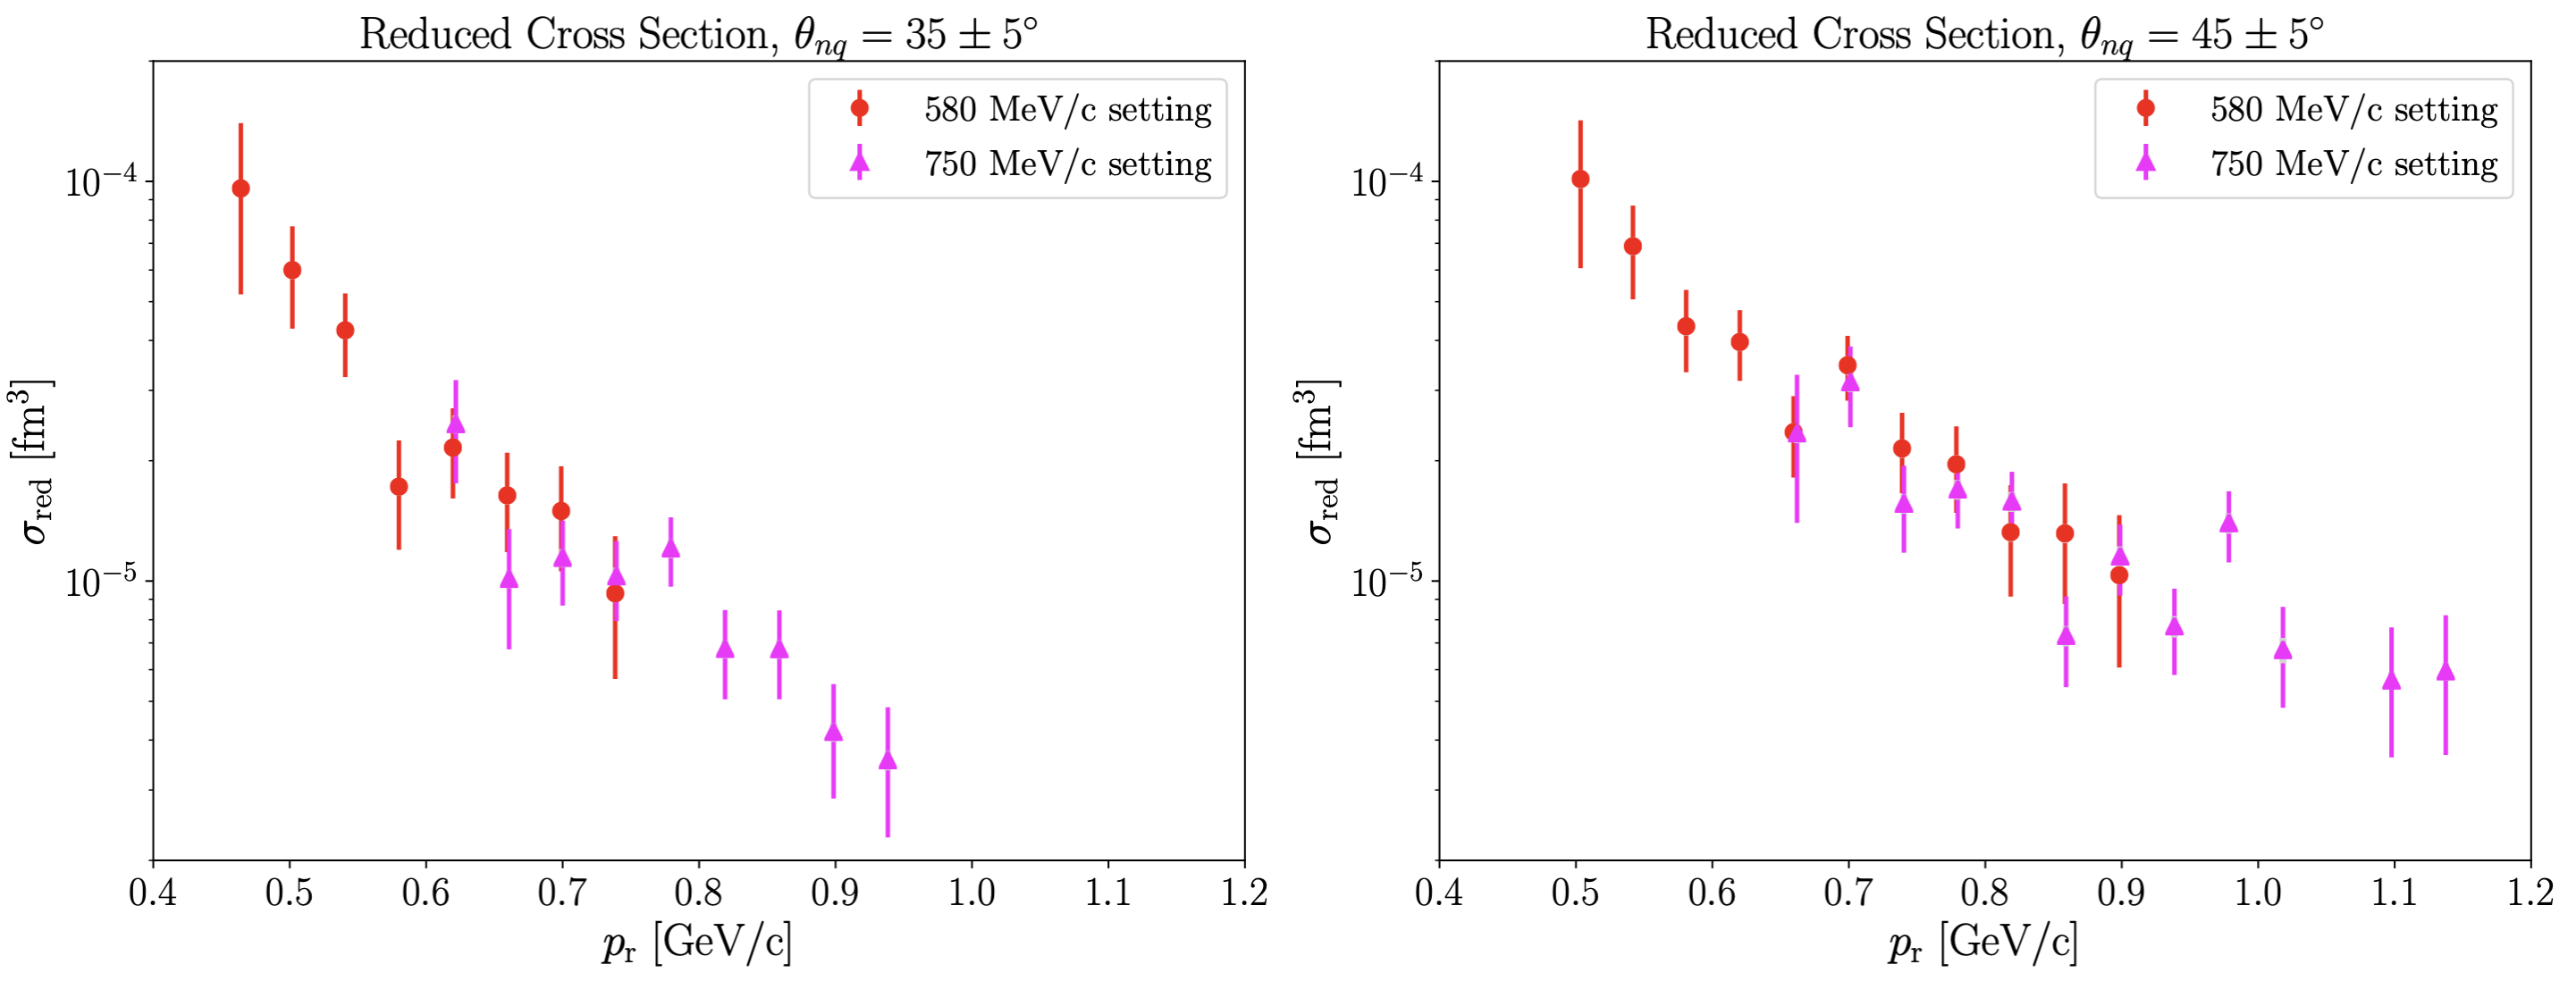
\includegraphics[scale=0.30]{RedXsec_overlap.png}
\caption{Reduced cross section overlap region between the 580 and 750 MeV/c settings. The 750 MeV/c setting data points have been offset right by +0.01 GeV/c for ease of comparison.}
\label{fig:RedXsec_overlap}
\end{figure}
\section{\large Radiative \& Bin-Centering Corrections}
\indent The radiative corrections were applied by multiplying the ratio of non-radiative to radiative SIMC yields to the data yield for each ($\theta_{nq}$, $p_{\mathrm{r}}$)
kinematic bin as described in the Letter. The radiative correction factors for $\theta_{nq}=35^{\circ}$ and $45^{\circ}$ are shown in Fig. \ref{fig:RC_factor}. The calculation was done using the
Laget PWIA and FSI models for systematic effect studies, but the FSI model was ultimately used to correct the data yield. \\
\indent The uncertainty in the radiative
correction factor was determined for each ($\theta_{nq}$, $p_{\mathrm{r}}$) bin by the Monte-Carlo statistics from the simulation and was propagated to the final cross section error.
The large uncertainty in the lowest momentum bin, $p_{\mathrm{r}} = 0.02\pm0.02$, can be understood from the fact that statistics were limited in this phase space region as indicated by
the "hole" observed at $p_{\mathrm{r}} = 0.02$ in Fig. \ref{fig:Pm_Ps} (right). 
\begin{figure}[!h]
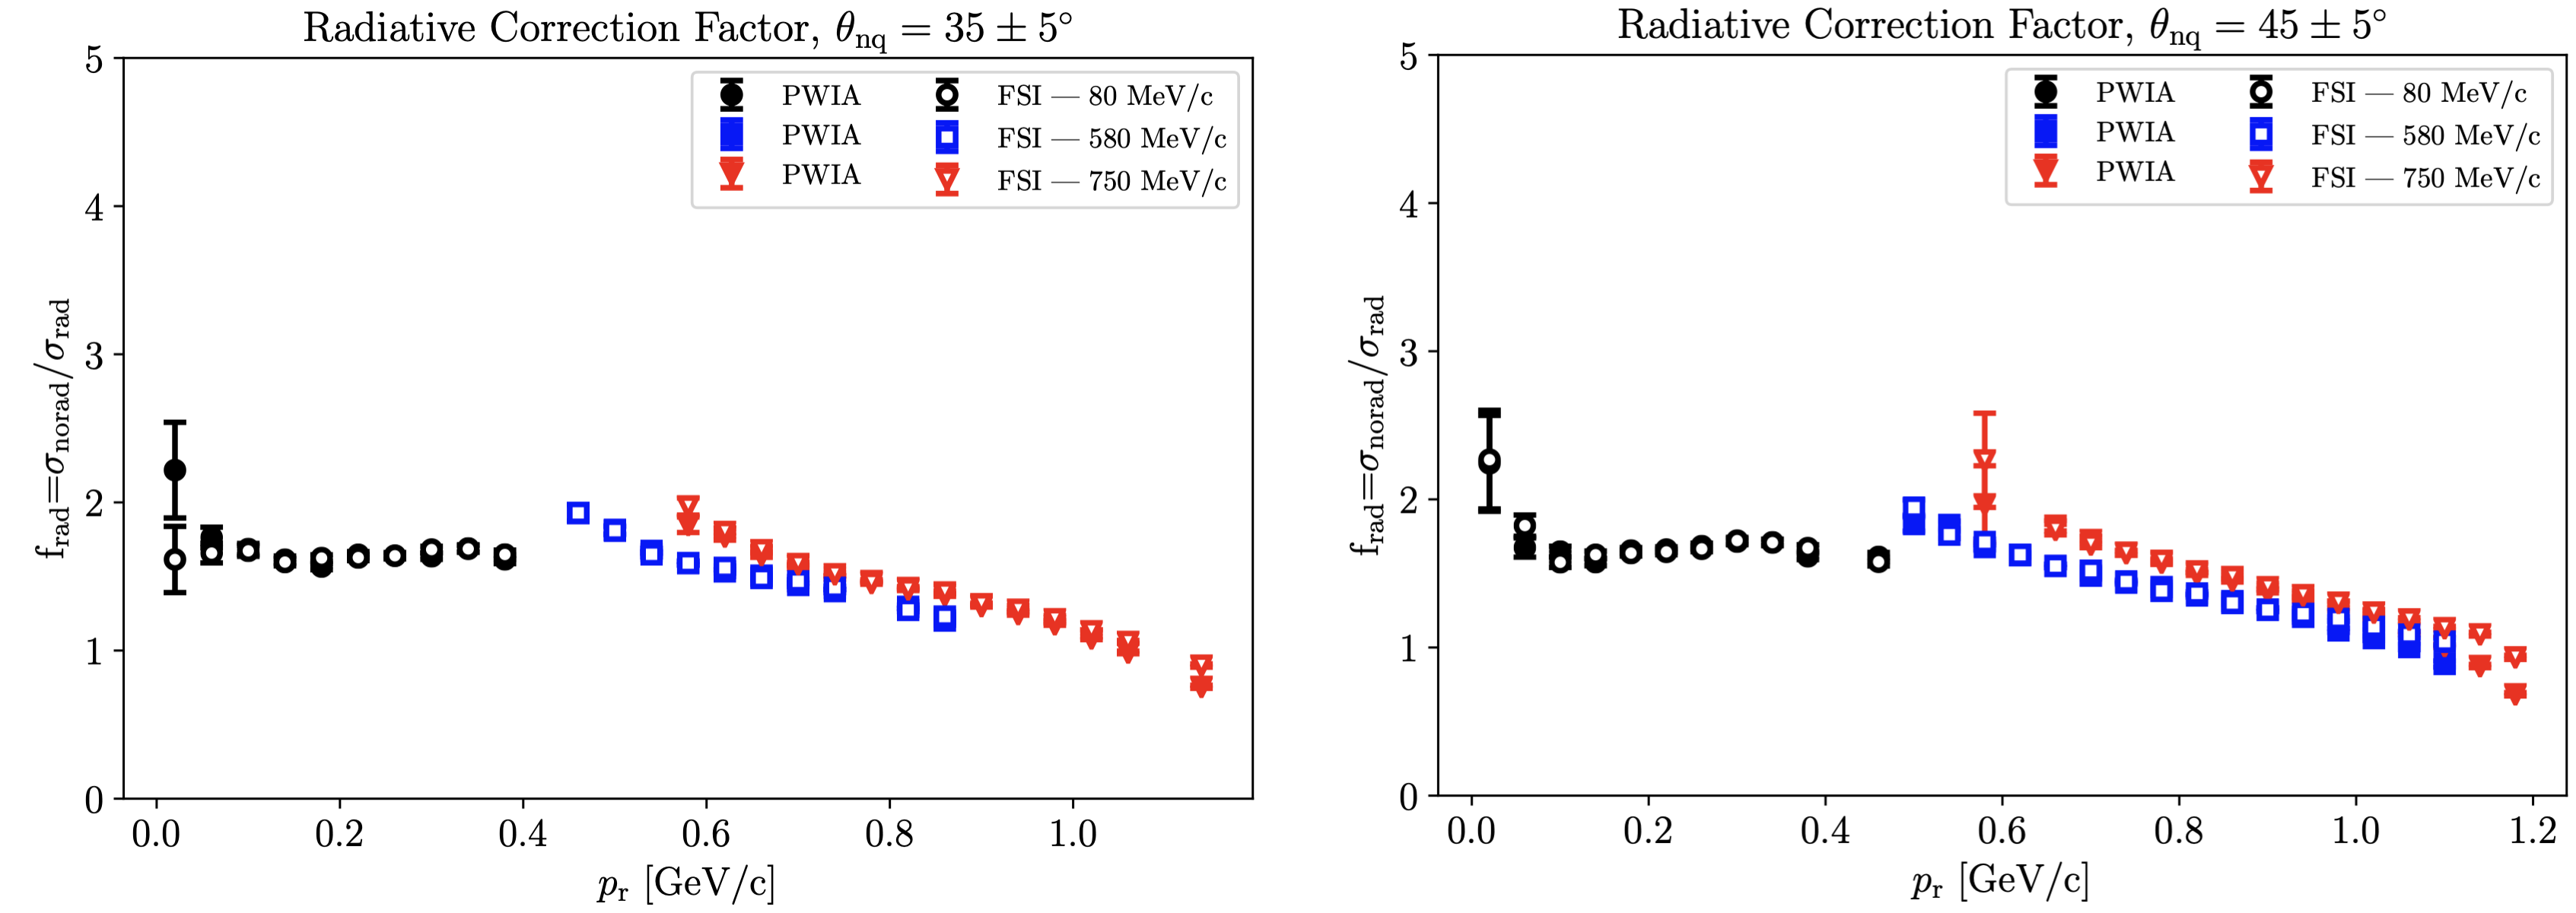
\includegraphics[scale=0.27]{RC_factor.png}
\caption{Radiative correction factor versus neutron recoil momenta, $p_{\mathrm{r}}$, for $\theta_{nq}=35^{\circ}$ (left) and $45^{\circ}$ (right). }
\label{fig:RC_factor}
\end{figure}\\
The bin centering corrections were applied by multiplying the ratio, $f_{\mathrm{bc}} \equiv \sigma_{\mathrm{avg.kin}}/\bar{\sigma}$, to the average data cross section over each ($\theta_{nq}$, $p_{\mathrm{r}}$)
kinematic bin, as described in the Letter. The bin centering correction factors for $\theta_{nq}=35^{\circ}$ and $45^{\circ}$ are shown in
Fig. \ref{fig:BC_factor}. The calculation was done using the Laget PWIA and FSI models for systematic effect studies, but the FSI model was ultimately used to correct the data cross section. \\
\begin{figure}[!ht]
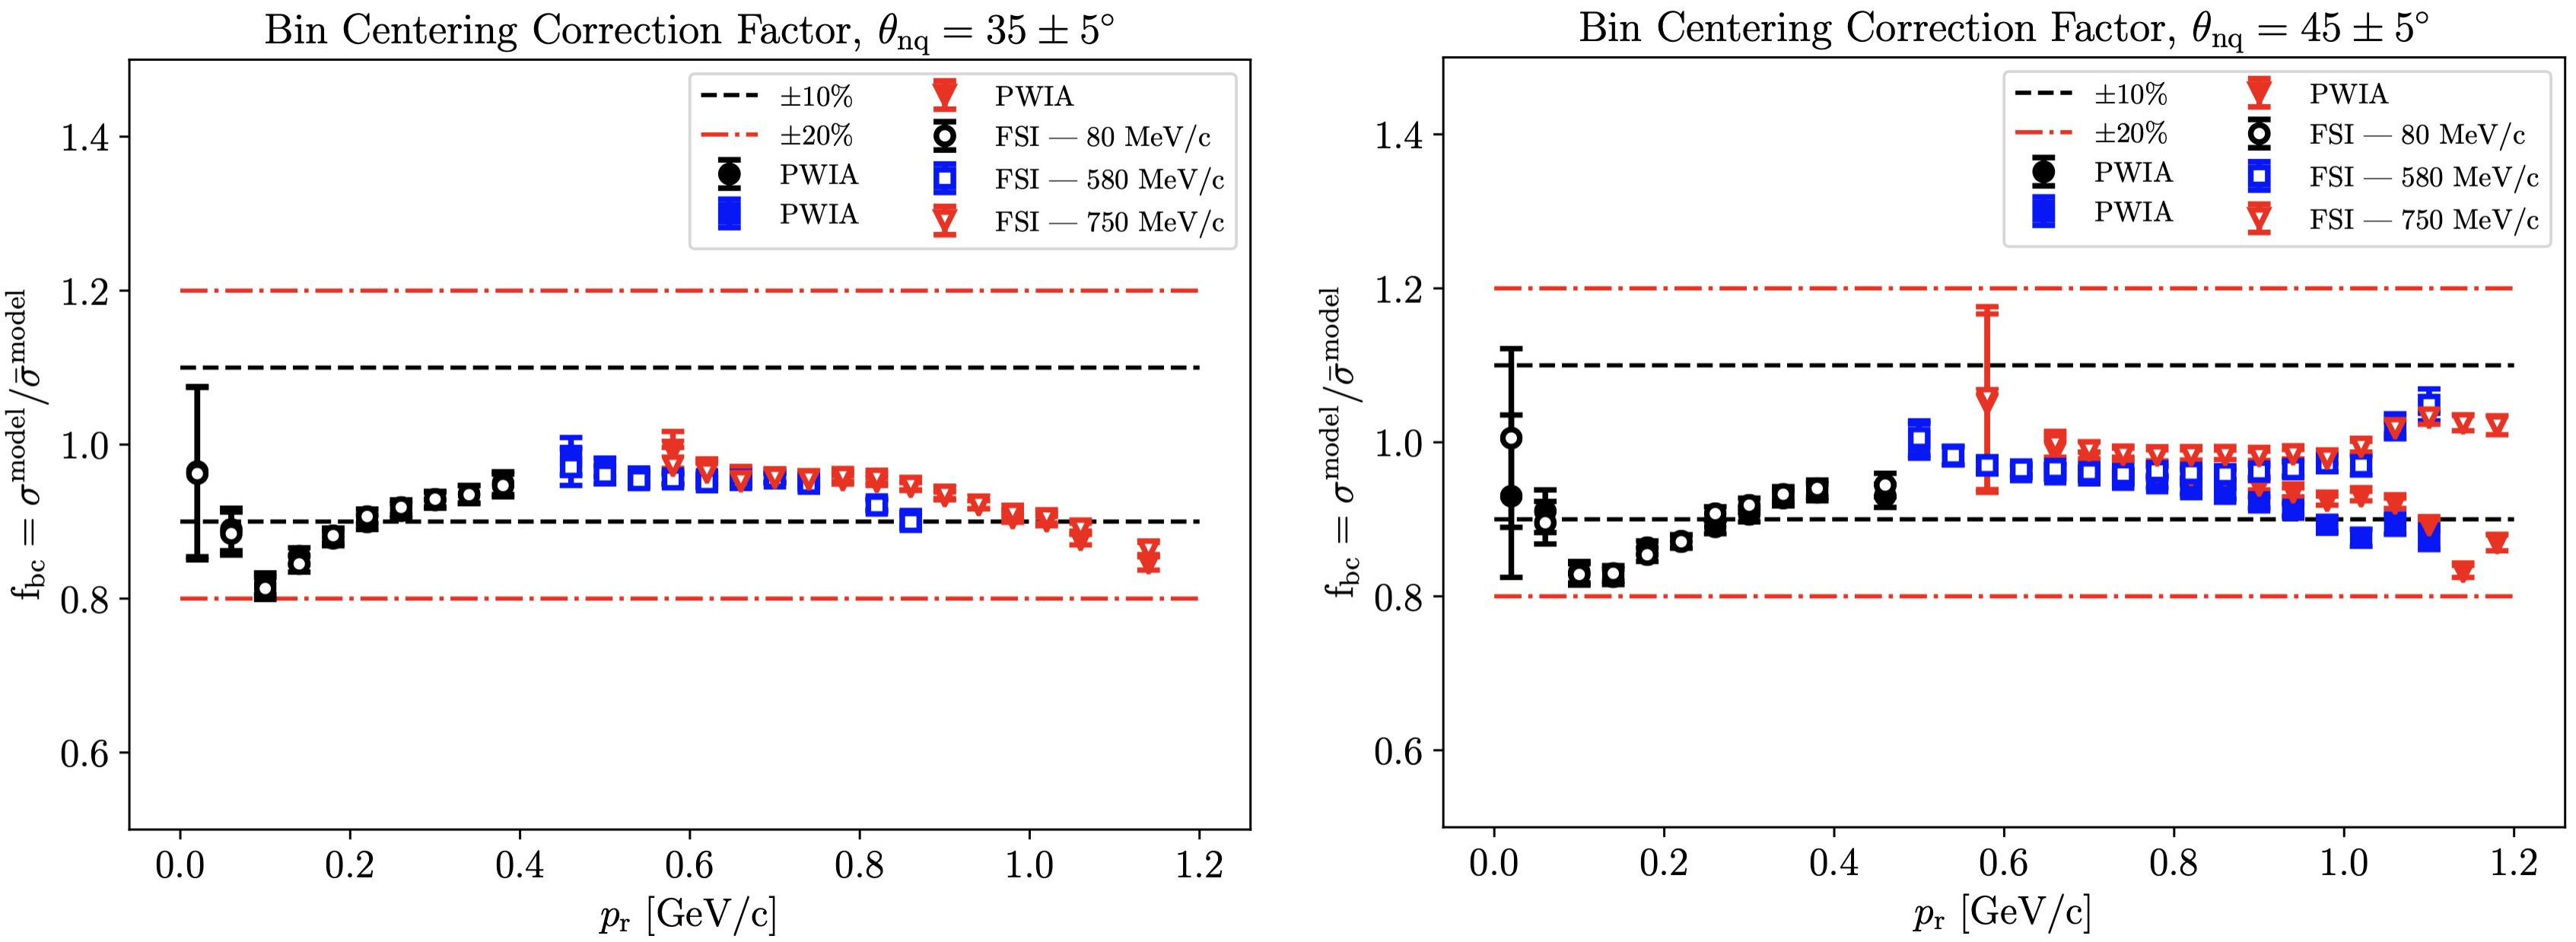
\includegraphics[scale=0.27]{BC_factor.png}
\caption{Bin centering correction factor versus neutron recoil momenta, $p_{\mathrm{r}}$, for $\theta_{nq}=35^{\circ}$ (left) and $45^{\circ}$ (right).
  The inner (black dashed) and outer (red dash-dotted) lines represent a percent deviation from unity of $\pm10\%$ and $\pm20\%$, respectively.}
\label{fig:BC_factor}
\end{figure}\\
\indent The uncertainty in the bin-centering correction factor was determined for each  ($\theta_{nq}$, $p_{\mathrm{r}}$) bin
using the standard error propagation for a ratio of two quantities and the result was propagated to the final cross section error. \\
\section{\large Systematic Uncertainty Studies on Radiative and Bin-Centering Corrections }
\indent The systematic effect on the cross sections due to model dependency of the radiative and bin-centering corrections was investigated (see Section 5.10 of Ref. \cite{cyero_phdthesis})
using the Barlow ratio approach \cite{barlow2002systematic,barlow2017}. In this case, the ratio was calculated from the difference between the experimental cross
sections using the Laget PWIA and FSI models for both radiative and bin-centering corrections. Figures \ref{fig:rad_sys} and \ref{fig:bc_sys}
show the Barlow ratio for radiative and bin-centering systematics is mostly within 2 standard deviations which show that
the model dependency of the correction factors have a negligible effect on the experimental cross sections.
\begin{figure}[!h]
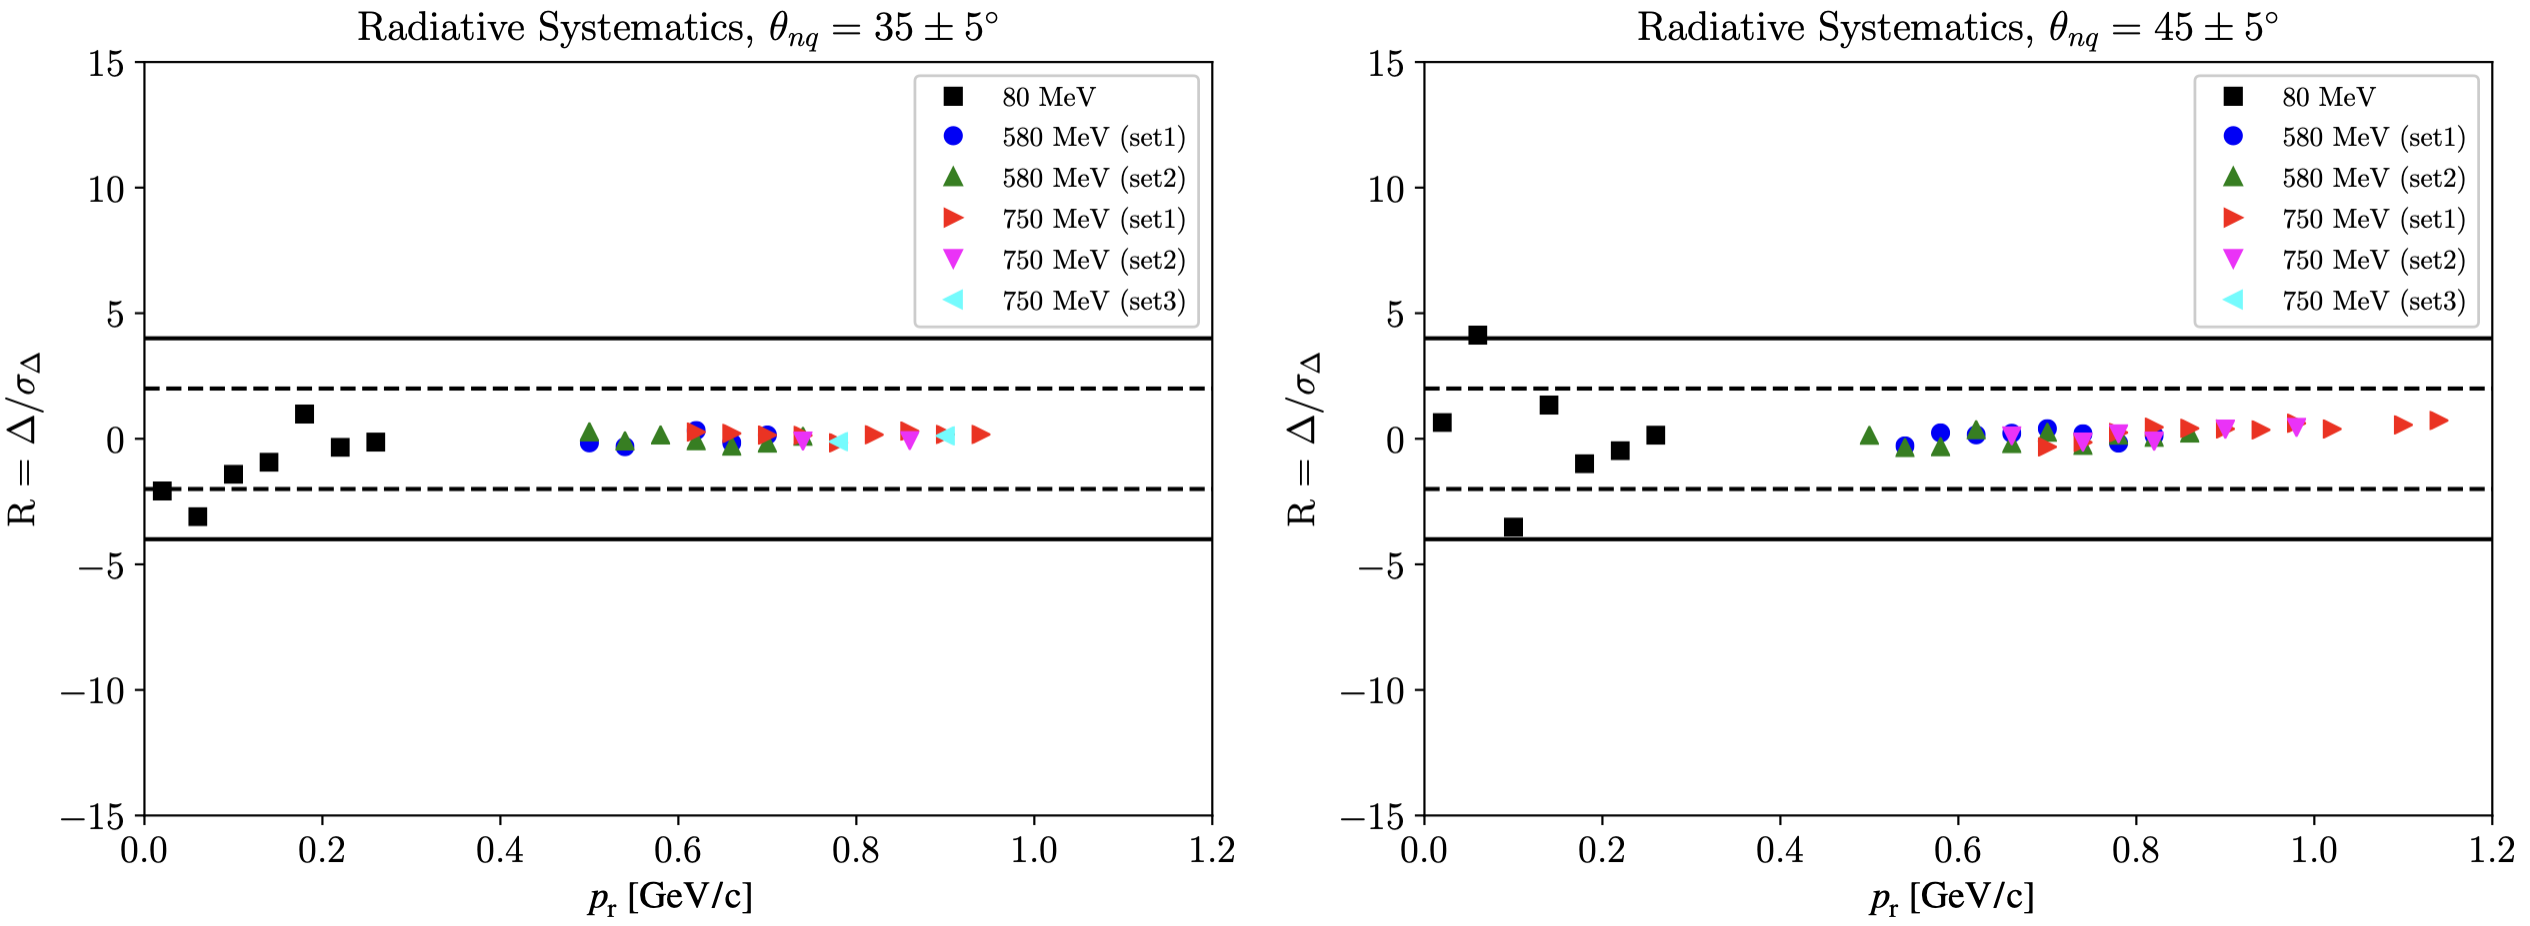
\includegraphics[scale=0.37]{rad_sys.png}
\caption{Systematic effects of the radiative corrections model dependency on the data cross sections
  for $\theta_{nq}=35^{\circ}$ (left) and $45^{\circ}$ (right). The inner (black dashed) and outer (black solid)
  lines represent the $\Delta=\pm2\sigma_{\Delta}$ and $\pm4\sigma_{\Delta}$ boundaries, respectively.  }
\label{fig:rad_sys}
\end{figure}
\begin{figure}[!ht]
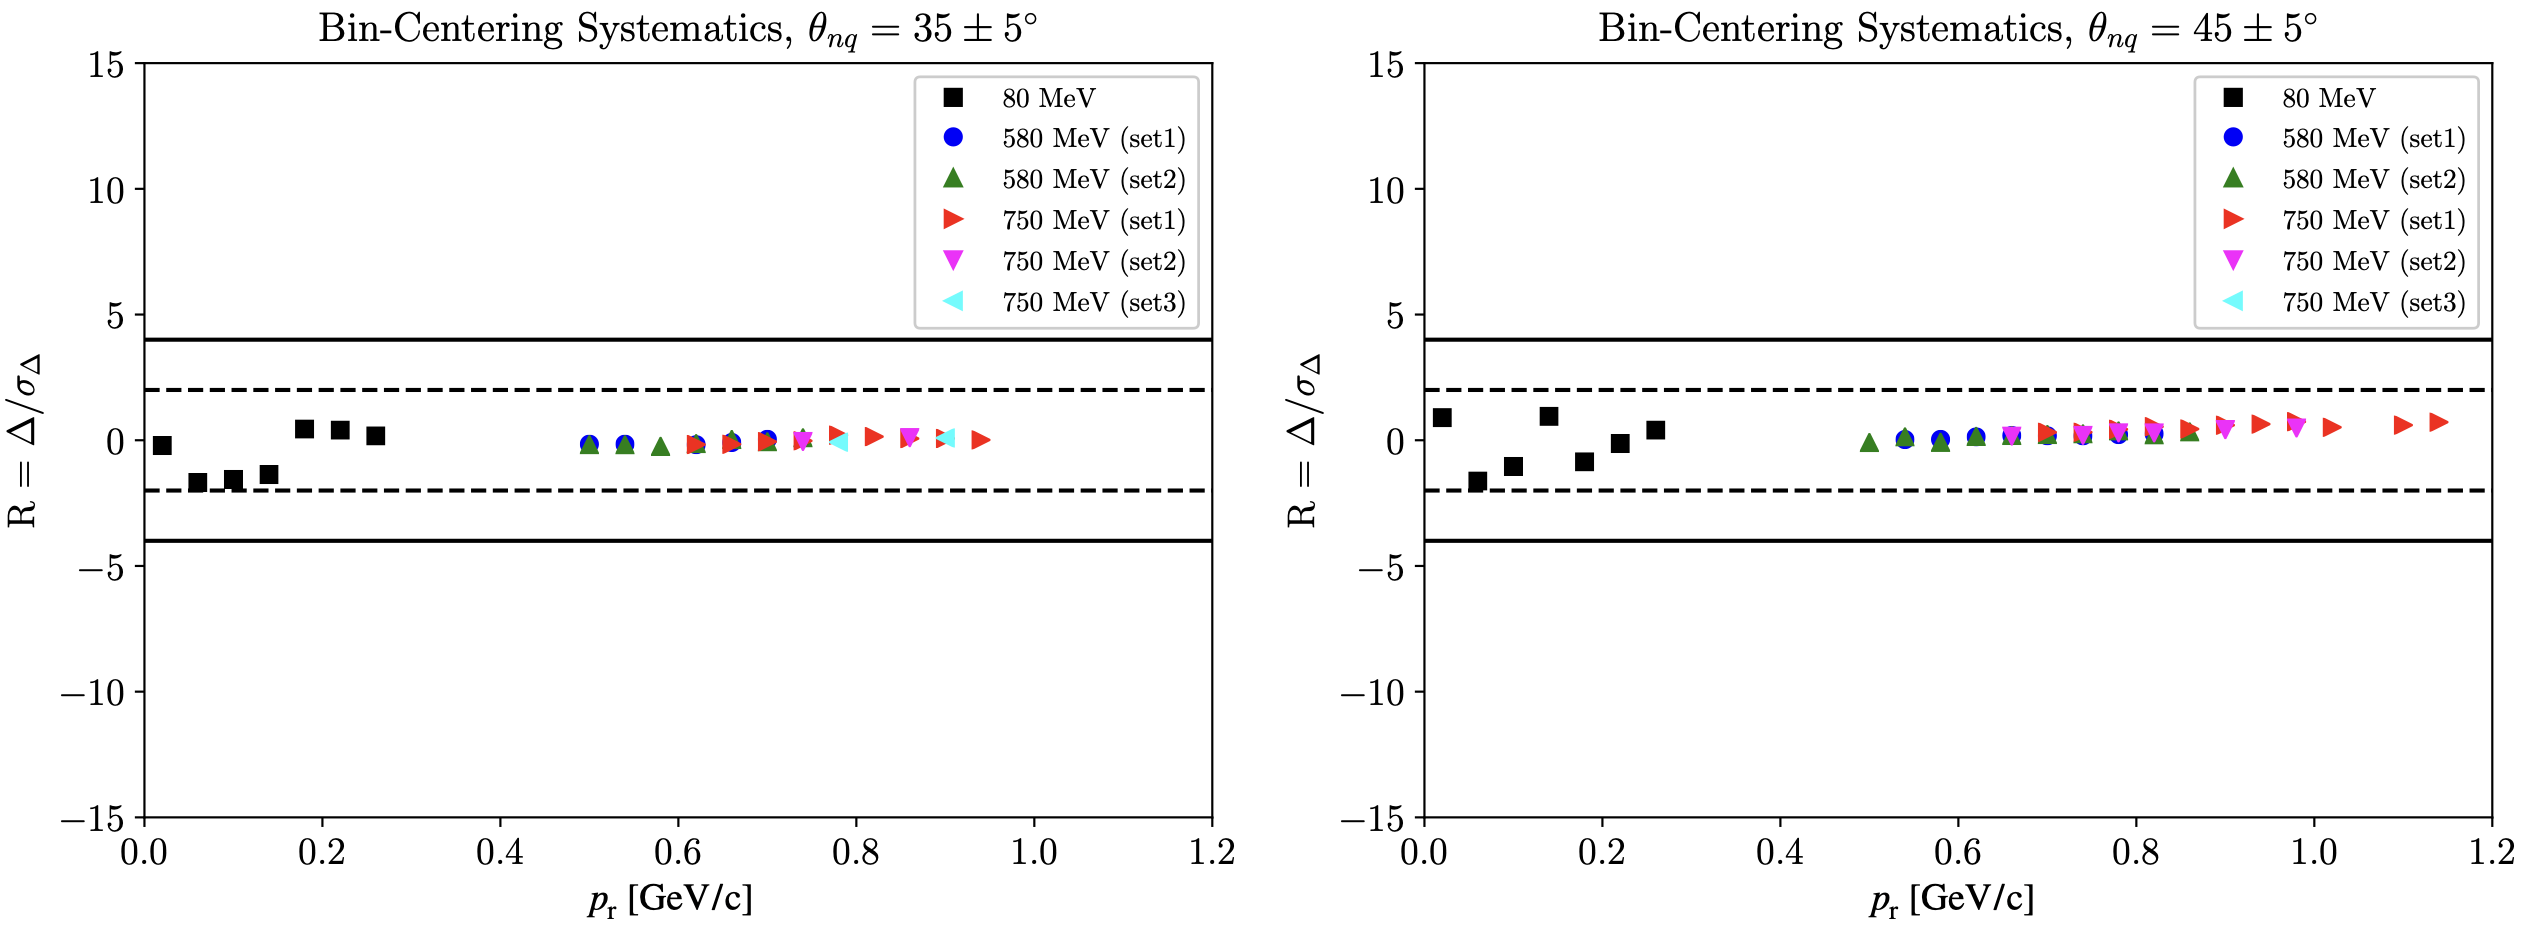
\includegraphics[scale=0.37]{bc_sys.png}
\caption{Same as Fig. \ref{fig:rad_sys} but for bin-centering correction systematics.}
\label{fig:bc_sys}
\end{figure}\\
\indent Systematic studies of the event selection cuts described above were also carried out using the R. Barlow approach. The studies demonstrated that variations in the software had a negligible
effect in the measured cross sections and thus no systematic uncertainties due to software cuts were included in the final result. For a detailed discussion of these studies see Section 5.10 of Ref. \cite{cyero_phdthesis}.
\\\\
\bibliography{supp}

\end{document}
